\documentclass[12pt]{report}
\usepackage[utf8]{vietnam}
\usepackage{amsmath}
\usepackage{amsfonts}
\usepackage{amssymb}
\usepackage{acronym}
\usepackage{graphicx}
\usepackage{caption}
\usepackage{booktabs}
\usepackage{hyperref}
\usepackage[useregional]{datetime2}
\usepackage{sectsty}
\usepackage{indentfirst}
\usepackage{bm}
\chapterfont{\centering}

\newcommand{\argmax}{\arg\!\max}

\begin{document}

\begin{titlepage}
\centering
{\large ĐẠI HỌC QUỐC GIA THÀNH PHỐ HỒ CHÍ MINH\\}
{\large TRƯỜNG ĐẠI HỌC BÁCH KHOA\\}
{\large CHƯƠNG TRÌNH KỸ SƯ CHẤT LƯỢNG CAO VIỆT PHÁP\\}
{\large KHOA ĐIỆN - ĐIỆN TỬ\\}
{\large BỘ MÔN VIỄN THÔNG}

\begin{figure}[h]
  \centerline{\includegraphics[scale=0.1]{images/logo_bk.png}}
\end{figure}

\vspace{0.3cm}

{\Large LUẬN VĂN TỐT NGHIỆP}

\vspace{0.7cm}

{\LARGE\bfseries HỆ THỐNG GIÁM SÁT VIỆC SỬ DỤNG THIẾT BỊ BẢO HỘ CÁ NHÂN ỨNG DỤNG MẠNG HỌC SÂU}

\vspace{0.7cm}

{\large\bfseries NGUYỄN THÁI SƠN - 1512847}

\vspace{0.7cm}

{\large GIẢNG VIÊN HƯỚNG DẪN:\\}
{\large\bfseries PGS. TS. HÀ HOÀNG KHA}

\vfill

{\itshape Thành phố Hồ Chí Minh, tháng 6 năm 2020}
\end{titlepage}

%
\chapter*{LỜI CẢM ƠN}
Khoảng thời gian học tập và rèn luyện tại \textbf{Trường Đại học Bách Khoa
Thành phố Hồ Chí Minh} đã trang bị cho em rất nhiều kiến thức hữu ích và cần thiết
về chuyên môn và xã hội để em có thể trở thành một công dân tốt và một kỹ sư
có năng lưc. Con đường học tập ở đại học trong suốt 5 năm vừa qua là không 
hề dễ dàng với muôn vàn thử thách và khó khăn. Để vượt qua những rào cản ấy, bên 
cạnh sự cố gắng của bản thân em còn là sự ủng hộ và giúp đỡ tận tình của quý \textbf{Thầy Cô}, 
\textbf{Gia đình} và \textbf{Bạn bè}. Em xin gửi lời cảm ởn chân thành và sâu sắc nhất 
đến quý \textbf{Thầy Cô Trường Đại học Bách Khoa Thành phố Hồ Chí Minh}, quý 
\textbf{Thầy Cô Khoa Điện – Điện Tử}, những người đã đi cùng với tri thức và 
tâm huyết truyền đạt vốn kiến thức quý báu của mình cho chúng em.

Em muốn giành riêng lời cảm ơn đặc biệt cho Thầy hướng dẫn của mình
– PGS. TS. Hà Hoàng Kha – người đã luôn tận tình hướng dẫn và giúp đỡ em trong
quá trình thực hiện luận văn này.

Ngoài ra, em cũng muốn giành cho gia đình và bạn bè lời cảm ơn chân thành và đặc
biệt là ba mẹ và ông bà em, những người đã luôn là chỗ dựa tinh thần vững chắc 
cho em trong nhưng thời điểm khó khăn.

Trong quá trình thực hiện luận văn chắc chắn không thể tránh khỏi những sai
sót, em rất mong nhận được những ý kiến đóng góp quý báu của quý Thầy
Cô để em có thể học hỏi thêm nhưng điều tốt đẹp và hoàn thiện luận văn của mình.
Sau cùng, em xin kính chúc quý \textbf{Thầy Cô Trường Đại học Bách Khoa Thành
phố Hồ Chí Minh} và \textbf{Thầy Hà Hoàng Kha} dồi dào sức khỏe, đạt được nhiều thành
công trong cuộc sống và luôn giữ vững niềm đam mê nghiên cứu và giảng dạy để có thể
tiếp tục truyền lửa tri thức cho những thế hệ sau.

\hfill
Thành phố Hồ Chí Minh, tháng 6 năm 2020

\vspace{0.5cm}

\hfill
Nguyễn Thái Sơn

\chapter*{TÓM TẮT LUẬN VẶN}
Ý tưởng về việc kết hợp trí tuệ nhân tạo và thị giác máy tính để ứng dụng vào các bài 
toán giám sát đã xuất hiện từ lâu. Tuy nhiên chỉ đến những năm gần đây khi các thiết bị
phần cứng có thể đáp ứng được yêu cầu về tính kĩ thuật và kinh tế thì các ứng dụng 
sử dụng các công nghệ này mới dần trở nên phổ biến. Một trong những ứng dụng đang rất được 
quan tâm là đảm bảo an toàn lao động của công nhân xây dựng thông qua một hệ thống giám 
sát sử dụng camera và trí tuệ nhân tạo để theo dõi việc sử dụng các thiết bị bảo hộ lao 
động của những người làm việc trong công trường.

Trong khuôn khổ của luận văn này, hệ thống giám sát việc sử dụng thiết bị bảo hộ cá nhân 
sẽ tập trung vào ba thiết bị thường gặp trong công trường xây dựng: mũ cứng, áo dạ quang 
bảo hộ và khẩu trang. Hệ thống sử dụng phương pháp phát hiện và phân loại vật thể YOLO, 
được xây dựng trên cơ sở mạng tích chập - CNN. Khi hoạt động, hệ thống sẽ có thể phát hiện 
và phân loại việc sử dụng các thiết bị bảo hộ lao động của công nhân ở công trường. Nếu phát 
hiện một trường hợp không sử dụng thiết bị bảo hộ lao động đang được theo dõi thì hệ thống 
sẽ gửi cảnh báo cho quan sát viên để kiểm tra và nhắc nhở. Việc này sẽ hỗ trợ rất nhiều trong 
công tác đảm bảo an toàn lao động trong xây dựng.

Hệ thống được viết bằng ngôn ngữ Python, mô hình máy học YOLOv3 và thư viện thị giác máy tính 
OpenCV.

%
\tableofcontents

%
\listoffigures

\listoftables

\chapter*{Danh sách từ viết tắt}
\begin{acronym}
\acro{MRC}{Maximal Ratio Combining}
\end{acronym}

%
\chapter{Giới thiệu}
\pagenumbering{arabic}
\setcounter{page}{1}
\section{Đặt vấn đề}
Ngành xây dựng luôn được coi là một trong những ngành ẩn chưa nhiều rủi ro về tai nạn lao động và khả năng mắc các bệnh nghề nghiệp. Trên thực tế nhiều vụ tai nạn nghiêm trọng đã xảy ra, lấy đi sinh mang hoặc để lại những thương tật nặng nề cho người lao động khiến họ mất khả năng làm việc, sinh hoạt như người bình thương. Kéo theo đó là nỗi đau về tinh thần và gánh nặng về kinh tế cho những thành viên trong gia đình người bị nạn. Do đó vấn đề đảm bảo an toàn vệ sinh lao động luôn là một trong những vấn đề được quan tâm hàng đầu ở các cấp, các ngành. Theo báo cáo của 63/63 tỉnh, thành phố trực thuộc Trung ương\cite{tnld:2019:gov}, trong năm 2019, trên toàn quốc xảy ra \textbf{7130} vụ tai nạn lao động với \textbf{7267} người bị nạn với thống kê theo bảng \ref{table:tnld_stats}.
\begin{center}

  \begin{tabular} {l l}
  \toprule
  \midrule

  Số người chết & 610 người\\
  Số vụ tai nạn lao động làm chết người & 572 vụ\\
  Số người bị thương nặng & 1592 người \\
  Nạn nhân là lao động nữ & 2535 người \\
  Số vụ tai nạn lao động có hai người bị nạn trở lên & 119 vụ \\
          
  \bottomrule
  \end{tabular}

\captionof{table}{Số liệu về tình hình tại nạn lao động năm 2020.
\label{table:tnld_stats}}
\end{center}

Một trong những nguyên nhân chính gây ra những vụ tai nạn thương tâm là việc người lao động không sử dụng trang thiết bị bảo hộ cá nhân trong quá trình lao động. Vấn đề này không chỉ xuất phát từ sự chủ quan của cá nhân người lao động mà còn ở sự thiếu sót, lỏng lẻo trong quá trình giám sát công trình của nhà thầu và người sử dụng lao động. Bảng \ref{table:tnld_reason} cho thấy các nguyên nhân chính dẫn đến tai nạn lao động gây chết người trong năm 2019.
\begin{center}

  \begin{tabular} {l l l}
  \toprule
  \it Nguyên nhân & \it \% tổng & \it \% tổng số \\
   & \it số vụ & \it người chết \\
  \midrule
  \it Do người sử dụng lao động & \it 47.74 & \it 49.99 \\
  \\
  \bf {\tab Người sử dụng lao động không xây dựng} & \bf 24.32 & \bf 26.27 \\ \bf{\tab quy trình, biện pháp làm việc an toàn} \\
  \\
  \bf {\tab Người sử dụng lao động không huấn luyện} \\ \bf {\tab an toàn lao động hoặc huấn luyện an toàn,} & \bf 14.41 & \bf 13.56 \\ \bf {\tab vệ sinh lao động chưa đầy đủ cho người} \\ \bf {\tab lao động}\\
  \\
  \bf {\tab Do tổ chức lao động và điều kiện lao động} & \bf 7.21 & \bf 8.47 \\
  \\
  \bf {\tab Thiết bị không đảm bảo an toàn lao động} & \bf 1.8 & \bf 1.69 \\
  \\
  \textit{\textbf{Do người lao động vi phạm quy trình quy}} & \textit{\textbf{14.41}}  & \textit{\textbf{14.41}} \\ \textit{\textbf{chuẩn an toàn lao động}} \\
  \\
  \it {Nguyên nhân khách quan khác, khó tránh} & \it 37.85 & \it 35.6 \\
  \bottomrule
  \end{tabular}

\captionof{table}{Các nguyên nhân chính dẫn đến tai nạn chết người.
\label{table:tnld_reason}}
\end{center}

Đối với người lao động, những điều kiện khắc nghiệt của môi trường làm việc như nhiệt độ ngoài trời cao hay thường xuyên phải vận động mạnh khiến đổ mồ hôi liên tục đã khiến họ chấp nhận đánh đổi sự an toàn của bản thân để đổi lấy sự thoải mái. Còn đối với những người giám sát công trình, họ không thể bao quát được toàn bộ quá trình làm việc tại các nơi làm việc khác nhau, do đó không thể nhắc nhở người lao động kịp thời trước khi xảy ra những tai nan mà hậu quả là có thể tránh khỏi hoặc được giảm nhẹ nếu người lao động có sử dụng trang thiết bị bảo hộ cá nhân.

Để tăng cường năng lực thực hiên đảm bảo an toàn vệ sinh lao động ở các công trình, nhiều chủ đầu tư và nhà thầu đã tiến hành lắp đặt các hệ thống camera giám sát quá trình làm việc. Các hệ thống này giúp giám sát viên có thể quan sát nhiều vị trí một lúc mà không cần phải di chuyển qua các địa điểm khác nhau trong công trình, giảm thiểu chi phí và thời gian thực hiên các công tác an toàn. Tuy nhiên, khi số lượng các khu vực cần quan sát tăng lên hoặc những người chịu trách nhiệm quan sát không tập trung vào nhiệm vụ  thì việc giám sát thông qua màn hình dễ xảy ra sai sót. Việc tích hợp công nghê AI vào các hệ thống giám sát sẽ là sẽ tăng thêm độ tin cậy cho công tác đảm bảo an toàn, giảm thiểu những sai sót không đáng có.

\section{Mục tiêu nghiên cứu}
Mục tiêu của luận văn là xây dựng, đánh giá một hệ thống nhận diện việc sử dụng thiết bị bảo hộ cá nhân của người lao động trong công trường. Khi phát hiện ra các trường hợp không sử dụng các trang thiết bị bảo hộ thì hệ thống sẽ đưa ra cảnh báo.  

\section{Phạm vi nghiên cứu}
Phạm vi của luận văn là tiến hành nhận dạng trên các video trích xuất từ camera. Mô hình nhận diện được huấn luyện sử dụng framework được xây dựng sẵn. Tập dữ liệu sử dụng để huấn luyện và đánh giá mô hình nhận diện được thu thập và dán nhãn bởi người làm luận văn. Một phần hình ảnh trong tập dữ liệu này có nguồn gốc từ các tập dữ liệu khác nhưng không sử dụng lại các nhãn của các tập dữ liệu đó. Các thiết bị bảo hộ cá nhân được tích hợp trong hệ thống gồm: mũ cứng, áo bảo hộ và khẩu trang.

\section{Phương pháp nghiên cứu}
Các giai đoạn trong quá trình nghiên cứu và hoàn thiện luận văn:
\begin{enumerate}
	\item Tìm hiều về CNN, mô hình YOLOv3 và cách ứng dụng của mô hình này vào việc nhận diện trang thiết bị bảo hộ lao động.
	\item Xây dựng tập dữ liệu gồm các hình ảnh chứa người đội nón bảo hộ, mặc áo phản quang và đeo khẩu trang cùng với tệp tin nhãn dán của từng hình.
	\item Huấn luyện mô hình nhận diện trên framework darknet và viết chương trình Python sử dụng mô hình đã huấn luyện để nhận diện.
	\item Đánh giá các thông số hiệu năng của mô hình đối với các thiết bị bảo hộ trong các trường hợp thực tế, kết luận và viết luận văn.
\end{enumerate}
YOLOv3 được chọn để làm mô hình nhận diện vì đây là một trong số các bộ nhận diện có hiệu năng cao trong thời gian thực, đã được sử dụng và đánh giá trên nhiều tập dữ liệu khác nhau.

\section{Cấu trúc luận văn}
Luận văn này bao gồm 5 chương. Chương 1 là chương mở đầu, giới thiệu bao quát về vấn đề, mục tiêu, phạm vi và phương pháp nghiên cứu luận văn. Chương 2 sẽ cung cấp những lý thuyết về các khái niệm được sử dụng trong luận văn. Chương 3 cho người đọc biết về cách tập dữ liệu được xây dựng, cách mô hình YOLOv3 được huấn luyện sử dụng framework darknet và cách xây dựng hệ thống sử dụng mô hình nhận diện. Chương 4 sẽ chứa những thông số đánh giá hiệu năng của bộ nhận diện và hệ thống trong các trường hợp khác nhau. Cuối cùng, trong chương 5 sẽ là các nhận xét về các kết quả đạt được và kết luận.\newpage\cleardoublepage
\chapter{Cơ sở lý thuyết}

\section{Gradient Descent}
Phần lớn các mô hình máy học được xây dựng dựa trên việc tối ưu hóa hàm mất mát hay nói cách khác là tìm cực tiểu của một hàm số biết trước. Đối với các hàm số đơn giản, việc xác đinh các điểm cực tiểu có thể được giải quyết thông qua việc tính toán đạo hàm cấp 1 và cấp 2. Tuy nhiên hàm mất mát của các mô hình máy học hay học sâu thường có số chiều lớn và đạo hàm phức tạp, do đó khó có thể áp dụng các phương pháp truyền thống để tìm các giá trị cực tiểu. Thay vào đó các mô hình này sử dụng giải thuật Gradient Descent để tìm các điểm cực tiểu của hàm mất mát.

Một hàm số có thể có nhiều điểm cực tiểu địa phương (local minimum) và cực tiểu toàn cục (global minimum). Ta có thể thấy trên hình \ref{fig:minimums} là đồ thị của một hàm số đơn biến, điểm màu xanh là cực tiểu địa phương, điểm màu đỏ là cực tiểu toàn cục.
\begin{figure}[ht!]
	\centerline{\includegraphics[scale=0.8]{images/minimums.png}}
  	\caption{Cực tiểu địa phương (màu xanh) và cực tiểu toàn cục (màu đỏ)}
  	\label{fig:minimums}
\end{figure}
Giả sử ta có hai điểm $M$ tại $x_M$ và $N$ tại $x_N$ trên đồ thị hình \ref{fig:minimums}, ta gọi điểm cực tiểu toàn cục là $G$. Lúc này ta muốn đưa điểm $M$ và $N$ về xấp xỉ hoặc trùng với vị trí của $G$ bằng giải thuật Gradient Descent. Ta nhận thấy $M$ nằm bên trái $G$ và $f^{'}(x_{M})<0$, nếu $M$ muốn di chuyển về phía $G$ thì $x_{M_{k+1}}=x_{M_{k}}+\delta$ tại bước thứ $k+1$. Ngược lại nếu ta muốn $N$ có $f^{'}(x_{N})>0$ tiến về phía $G$ tại bước tình toán thứ $k+1$ thì $x_{N_{k+1}}=x_{N_{k}}-\delta$. Như vậy để một điểm bất kì $(x,f(x))$ lân cận $G$ trên đồ thị tiến về $G$ thì vị trí của điểm đó phải được cập nhật sau mỗi bước tính toán bằng cách cộng với một lượng $\delta$ với $sign(\delta)=-sign(f^{'}(x))$. Trong thực thế, công thức được sử dụng có dạng:
\begin{equation}
	x_{k+1}=x_{k}-{\mu}f^{'}(x_{k})
\end{equation}
Với $\mu$ là \emph{tốc độ học}, ${\mu}{\in}{\mathbb{R}}$, ${\mu}>0$. Nếu ta chọn $\mu$ lớn thì ta sẽ cần ít số bước tính toán hơn để đến gần vị trí cực tiểu mong muốn nhưng trong nhiều trường hợp độ sai lêch giữa vị trí của điểm tính toán được sau cùng và vị trí của điểm cực tiểu sẽ tương đối cao. Ngược lại, nếu ta chọn $\mu$ nhỏ thì ta sẽ cần nhiều hơn số bước tính toán, bù lại khoảng cách giữa vị trí điểm tính toán được sau cùng và vị trí điểm cực tiểu sẽ có thể rất nhỏ.

Việc áp dụng giả thuật Gradient Descent lên làm đa biến là một sự mở rộng của ví dụ hàm đơn biến ở trên. Cho hàm số $f:{{\mathbb{R}}^n}{\rightarrow}{\mathbb{R}}, n{\in}{\mathbb{N}}^*$, ta cần tìm cực tiểu cho $f(X)$ với $X=\begin{pmatrix}x_0 & ... & x_{n-1}\end{pmatrix}, n{\in}{\mathbb{N}}^*$ từ một điểm khởi đầu $X_0$ bằng giải thuật Gradient Descent. Công thức để tính toán cho mỗi bước là:
\begin{equation}
	X_{k+1}=X_{k}-{\mu}{{\nabla}_X}f\left(X_{k}\right)
\end{equation}
\subsection{Batch Gradient Descent}
Giải thuật Batch Gradient Descent sử dụng tất cả các điểm đầu vào để cập nhật lại vector trọng số tại mỗi bước. Giả sử ta cần tối ưu hàm mất mát của một bài toán hồi quy tuyến tính gồm 30 điểm đầu vào với mỗi điểm gồm 2 tham số $\left(x,f\left(x\right)\right)$ ở hình \ref{fig:batch_gradient_descent}. Để tìm gradient cho mỗi điểm ta cần thực hiện 2 phép toán theo toán tử $\nabla$, đồng thời ta phải tìm gradient cho cả 30 điểm tại mỗi bước lặp và lấy trung bình của các kết quả này để cập nhật trọng số. Tổng số phép toán mà ta phải thực hiện cho tại mỗi bước là $30\times2=60$. Con số này sẽ tăng lên gấp nhiều lần đối với các bài toán thực tế khi số điểm và số tham số là vài triệu hoặc vài tỷ. Nói cách khác thuật toán này không hiệu quả về mặt tính toán với các bài toán máy học với dữ liệu lớn và phải cập nhật liên tục.
\begin{figure}[ht!]
	\centerline{\includegraphics[scale=0.6]{images/batch_gradient_descent.png}}
  	\caption{Batch Gradient Descent với bài toán hồi quy tuyến tính. Toàn bộ số điểm đầu vào đều được dùng để cập nhật các vector trọng số $(a,b)$ cho đường hồi quy tại mỗi bước, với $a$ là độ dốc và $b$ độ sai lệch.}
  	\label{fig:batch_gradient_descent}
\end{figure}
Ngoài ra sau khi đã tìm được nghiêm tối ưu của bài toán. Nếu ta thêm một điểm đầu vào mới vào tập dữ liệu cũ thì việc tính toán phải thực hiện lại từ đầu với toàn bộ điểm đầu vào bao gồm tập điểm đầu vào cũ và điểm mới thêm vào.
\subsection{Stochastic Gradient Descent}
Khác với Batch Gradient Descent giải thuật Stochastic Gradient Descent chỉ dùng gradient của một điểm ngẫu nhiên để cập nhật lại vector trọng số tại mỗi bước. Sau khi đi qua hết tất cả các điểm của tập đầu vào, thứ tự các điểm sẽ được xáo trộn và giải thuật lại tiếp tục với từng điểm. Mỗi một lần giải thuật Stochastic Gradient Descent tính toán xong với một điểm được gọi là một \emph{iteration} còn với toàn bộ tập điểm thì gọi là một \emph{epoch}. Cũng bài toán hồi quy tuyến tính ở trên nhưng với giải thuật Stochastic Gradient Descent (hình \ref{fig:stochastic_gradient_descent}), ta có thể thấy số iteration mà giải thuật Stochastic Gradient Descent phải thực hiện trong một epoch là 30. Số phép tính của một lần tính toán là 2. 
\begin{figure}[ht!]
	\centerline{\includegraphics[scale=0.6]{images/stochastic_gradient_descent.png}}
  	\caption{Stochastic Gradient Descent với bài toán hồi quy tuyến tính. Một điểm đầu vào được chọn ngẫu nhiên để cập nhật các vector trọng số $(a,b)$ cho đường hồi quy tại mỗi iteration, với $a$ là độ dốc và $b$ độ sai lệch.}
  	\label{fig:stochastic_gradient_descent}
\end{figure}

Do gradient của 1 điểm chỉ là xấp xỉ gần đúng của trung bình gradient của cả tập điểm nên việc cập nhật tại mỗi iteration sẽ có sai số nhật định, đồng thời các giá trị gradient tính toán được có thể có sư dao động lớn do tập điểm đầu vào thường bị tác động bởi nhiễu. Trên thực tế thì kết quả của giải thuật này có mức độ tối ưu khá tốt và hiệu quả tính toán cao. Sau khi đã hoàn thành tính toán trên tập dữ liệu cũ, nếu như có những điểm mới được thêm vào thì ta chỉ cần chạy giải thuật với các điểm mới mà không cần phải chạy lại giải thuật với toàn bộ các điểm như Batch Gradient Descent.
\subsection{Mini-batch Gradient Descent}
Mini-batch Gradient Descent là sự kết hợp của Batch Gradient Descent và Stochastic Gradient Descent. Một mini-batch sẽ có $n$ điểm với $1<n{\leq}N$, $N$ là tống số điểm của tập dữ liệu đầu vào. Việc chia tập điểm ban đầu thành các batch sẽ được thực hiện một cách ngẫu nhiên. Mỗi một lần giải thuật xử lý xong một  batch sẽ là một iteration và sau khi tất cả các batch được xử lý thì sẽ là một epoch. Như vậy $no\_batch=\frac{N}{n}$. Phương pháp này cho kết quả gần với Batch Gradient Descent nhưng không dùng nhiều tài nguyên tính toán như Batch Gradient Descent và không cần phải lặp lại nhiều lần như Stochastic Gradient Descent.
\begin{figure}[ht!]
	\centerline{\includegraphics[scale=0.6]{images/mini_batch_gradient_descent.png}}
  	\caption{Mini-batch Gradient Descent với bài toán hồi quy tuyến tính. Một batch sẽ gồm ba điểm đầu vào được chọn ngẫu nhiên để cập nhật các vector trọng số $(a,b)$ cho đường hồi quy tại mỗi iteration, với $a$ là độ dốc và $b$ độ sai lệch. Một epoch sẽ gồm mười batch.}
  	\label{fig:mini_batch_gradient_descent}
\end{figure}
\subsection{Điều kiện dừng của giải thuật}
Ta đã biết các giải thuật Gradient Descent sẽ cần phải thực hiện rất nhiều vòng lặp tính toán để có thể hội tụ. Tuy nhiên rất khó để nói được khi nào có thể dừng được giải thuật. Trong thực tế có nhiều cách khác nhau được dùng để chọn số bước tính toán:
\begin{enumerate}
	\item Chọn một số lương vòng lặp nhất định dựa vào một số tiêu chí như số lượng dữ liệu đầu vào. Cách làm này có thể cho kết quả không đủ tốt, có thể nghiệm tối ưu nằm ở các bước trước hoặc sau điểm kết thúc.
	\item Kiểm tra sự thay đổi của hàm mất mát giữa hai lần cập nhật liên tiếp, nếu sự sai lêch đạt tới ngưỡng đủ nhỏ thì ngưng giải thuật. Tuy nhiên nếu trên đồ thị của hàm mất mát có một vùng bằng phẳng nhưng không phải là cực tiểu thì giải thuật sẽ dừng tại điểm này mà không đạt được cực tiểu.
	\item Kiểm tra sự thay đổi của gradient giữa hai lần cập nhật liên tiếp, nếu sự sai lêch đạt tới ngưỡng đủ nhỏ thì ngưng giải thuật. Nhược điểm của phương pháp này là việc tính gradient của các hàm phức tạp khó có thể thực hiện được.
	\item Kiểm tra kết quả của giải thuật để ngừng việc lặp. Việc này cần người thực hiện việc huấn luyên mô hình phải thường xuyên kiểm tra các tham số hiệu năng của giải thuật lên một tập dữ liệu kiểm tra - \emph{validation set} để xem tại thời điểm nào giải thuật có hiệu năng tốt nhất.
\end{enumerate}
\section{Backpropagation}
Xét một mô hình mạng neuron (hình \ref{fig:ann})
\begin{figure}[ht!]
	\centerline{\includegraphics[scale=0.6]{images/ann.png}}
  	\caption{Mô hình mạng neuron đơn giản.}
  	\label{fig:ann}
\end{figure}
Quá trình dữ liệu được đưa vào lớp đầu tiên cho đến khi có kết quả ở lớp sau cùng được gọi là quá trình \emph{feed-forward}.
\begin{align*}
	a^{(0)}&=x \\
	z^{(k)}&={\boldsymbol{W}^{(k)T}}{a^{(k-1)}}+{\boldsymbol{b}}^k,k=1,2,..,N \\
	a^{(l)}&=f^{(k)}\left(z^{(k)}\right),k=1,2,..,N \\
	\widehat{y}&=a^{(N)}
\end{align*}
Ta thấy với mô hình này, hàm mất mát $J\left({\boldsymbol{W}},{\boldsymbol{b}},{\boldsymbol{X}},{\boldsymbol{Y}}\right)$ sẽ phụ thuộc vào tập các ma trận trọng số $\boldsymbol{W}$ và tập các vector bias của mỗi lớp $\boldsymbol{b}$. Việc tính gradient của làm mất mát phụ thuộc vào việc tính các đạo hàm riêng ${\frac{{\partial}J}{{{\partial}\boldsymbol{W}}^{(k)}}}$; ${\frac{{\partial}J}{{\partial}\boldsymbol{b}^{(k)}}}$, ${\forall}k=1,2,..,N$. Đối với bài toán hồi quy tuyến tính thì hàm mất mát là hàm trung bình bình phương sai số (Mean Square Error - MSE), lúc này
\begin{equation}
	J
	\left(
		{\boldsymbol{W}},{\boldsymbol{b}},{\boldsymbol{X}},{\boldsymbol{Y}}
	\right)
	=
	{
		{\frac{1}{M}} 
		{\sum_{i=1}^{(M)}} 
		{ { {\parallel} y_i - \widehat{y_i} {\parallel} }_2 }^2
	}
	=
	{
		{\frac{1}{M}} 
		{\sum_{i=1}^{(M)}} 
		{ { {\parallel} y_i - {a_i}^{(N)} {\parallel} }_2 }^2
	}
\end{equation}
Với $N$ là số điểm trong tập điểm đầu vào. Ta nhận thấy để tìm các đạo hàm riêng của $J$ với ${\boldsymbol{W}}$ và ${\boldsymbol{b}}$ trong trường hợp này là rất khó vì phương trình của $J$ không phụ thuộc trực tiếp vào ${\boldsymbol{W}}$ và ${\boldsymbol{b}}$. Để có thể hiện thực các giải thuật thuộc họ Gradient Descent thì phương pháp thường được sử dụng là Backpropagation. Phương pháp này sẽ cập nhật các trọng số theo chiều từ layer cuối cùng đến layer đầu tiên. Đầu tiên giải thuật sẽ tính đạo hàm của hàm mất mát theo ma trận trọng số của lớp cuối cùng.
\begin{align*}
	\frac
		{ {\partial} J }
		{ {\partial} {w_{ij}^{(N)}} }
	&=
	\frac
		{ {\partial} J }
		{ {\partial} {z_{j}^{(N)}} }
	{\cdot}
	\frac
		{ {\partial} {z_{j}^{(N)}} }
		{ {\partial} {w_{ij}^{(N)}} } \\
	&=
	{e_{j}^{(N)}}
	{
		\frac
			{ {\partial} \left(
							{w_{ij}^{(N)T}}
							a^{(N-1)}
							+
							{b_{j}^{(N)}}
						 \right)
			}
			{ {\partial} {w_{ij}^{(N)}} }
	}\\
	&={e_{j}^{(N)}}{a_{i}^{(N-1)}}
\end{align*}
Với ${e_{j}^{(N)}}=\frac{{\partial}J}{{\partial}{z_{j}^{(N)}}}$ có thể tính được tương đối dễ dàng. Tương tự ta có đạo hàm riêng của $J$ với bias ở lớp cuối cùng.
\begin{align*}
	\frac
		{ {\partial} J }
		{ {\partial} {b_{j}^{(N)}} }
	&=
	\frac
		{ {\partial} J }
		{ {\partial} {z_{j}^{(N)}} }
	{\cdot}
	\frac
		{ {\partial} {z_{j}^{(N)}} }
		{ {\partial} {b_{j}^{(N)}} } \\
	&={e_{j}^{(N)}}
\end{align*}
Các công thức trên cũng đúng với một lớp bất kỳ trong mạng neuron. Ta lấy mô hình hai lớp liên tiếp của một mạng neuron ở hình \ref{fig:ann} để đưa ra công thức tổng quát như sau:
\begin{align*}
	\frac
		{ {\partial} J }
		{ {\partial} {w_{ij}^{(k)}} }
	&=
	\frac
		{ {\partial} J }
		{ {\partial} {z_{j}^{(k)}} }
	{\cdot}
	\frac
		{ {\partial} {z_{j}^{(k)}} }
		{ {\partial} {w_{ij}^{(k)}} } \\
	&=
	{e_{j}^{(k)}}
	\frac
		{ {\partial} \left(
						{w_{ij}^{(k)T}}
						a^{(k-1)}
						+
						{b_{j}^{(k)}}
					 \right)
		}
		{ {\partial} {w_{ij}^{(N)}} } \\
	&={e_{j}^{(k)}}{a_{i}^{(k-1)}} \\ \\
	\frac
		{ {\partial} J }
		{ {\partial} {b_{j}^{(k)}} }
	&=
	\frac
		{ {\partial} J }
		{ {\partial} {z_{j}^{(k)}} }
	{\cdot}
	\frac
		{ {\partial} {z_{j}^{(k)}} }
		{ {\partial} {b_{j}^{(k)}} } \\
	&={e_{j}^{(k)}}
\end{align*}
Ta sẽ tính $e_{j}^{(k)}$ như sau:
\begin{align*}
	{e_{j}^{(k)}}
	&=
	{\frac
		{ {\partial} J }
		{ {\partial} {z_{j}^{(k)}} }
	}
	=
	{\frac
		{ {\partial} J }
		{ {\partial} {a_{j}^{(k)}} }
	}
	{\cdot}
	{\frac
		{ {\partial} {a_{j}^{(k)}} }
		{ {\partial} {z_{j}^{(k)}} }
	} \\
	&=\left( 
			 {\sum_{l=1}^{d^{(k+1)}}} 
			 {\frac
			 	{ {\partial} J }
			 	{ {\partial} {z_{l}^{k+1}} } 
			 }
			 {\cdot}
			 {\frac
			 	{ {\partial} {z_{l}^{(k+1)}} }
			 	{ {\partial} {a_{j}^{(k)}} } 
			 }
		\right) 
		{
			{f^{(k)'}} \left( 
					{z_{j}^{(k)}} 
				 \right)
		} \\
	&=\left( 
			 {\sum_{l=1}^{d^{(k+1)}}} 
			 e_{l}^{(k+1)}
			 {\cdot}
			 w_{jl}^{(k+1)}
		\right) 
		{
			{f^{(k)'}} \left( 
					{z_{j}^{(k)}} 
				 \right)
		}
\end{align*}
Ta có $f:{\mathbb{R}}{\rightarrow}[0,1]$ là hàm kích (activation function) hay còn gọi là hàm bao tại một node trong mạng neuron, $a_{j}^{k}=f\left(z_{j}^{k}\right)$, do dó ta có đạo hàm riêng của $a_{j}^{k}$ theo $z_{j}^{k}$ chính là đạo hàm của $f$. Ngoài ra do $a_{j}^{k}$ trực tiếp tham gia vào việc tính các $z_{l}^{k+1},l=1,2,..,d^{(k+1)}$ nên ${\frac{{\partial}J}{{\partial}{a_{j}^{k}}}}$ có thể tách ra thành tổng của tích các đạo hàm riêng như dòng thứ hai. Tương tự như vậy ta có thể tính
\begin{equation}
	\frac
		{ {\partial} J }
		{ {\partial} {b_{j}^{(k)}} }
	= {e_{j}^{(k)}}
\end{equation}
Việc tính ${e_{j}^{k}}$ sẽ phụ thuộc vào kết quả của ${e_{j}^{k+1}}$ do đó phương pháp này được gọi là Backpropagation.
Các bước để thực hiện giải thuật Backpropagation cho một mạng neuron nhân tạo gồm:
\begin{enumerate}
	\item Feedforward: Với mỗi giá trị đầu vào của x, tính giá trị đầu ra của mạng neuron, đồng thời lưu lại các kết quả ${\boldsymbol{a}}^{(k)}$ tại mỗi lớp.
	\item Với mỗi node thứ $j$ ở lớp ngoài cùng tính
\begin{equation}
	{e_{j}^{(N)}}
	=
	\frac
		{ {\partial} J }
		{ {\partial} {z_{j}^{(N)}} }
\end{equation}
	\item Từ đó suy ra:
\begin{align*}
	\frac
		{ {\partial} J }
		{ {\partial} {w_{ij}^{(N)}} }
	&=
	{a_{i}^{(N-1)}}
	{e_{j}^{(N)}} \\
	\frac
		{ {\partial} J }
		{ {\partial} {b_{j}^{(N)}} }
	&=
	{ e_{j}^{(N)} }
\end{align*}
	\item Với $k=N-1,N-2,...,1$ tìm $e_{j}^{(k)}$
\begin{equation}
	e_{j}^{(k)}
	=
	\left( 
		{\sum_{l=1}^{d^{(k+1)}}}
		e_{l}^{(k+1)}
		{\cdot}
		w_{jl}^{(k+1)}
	\right) 
	{
		{f^{(k)'}} 
		\left( 
			{z_{j}^{(k)}} 
	 	\right)
	}
\end{equation}
	\item Cập nhật đạo hàm cho từng trọng số và bias:
\begin{align*}
	\frac
		{ {\partial} J }
		{ {\partial} {w_{ij}^{(k)}} }
	&=
	{a_{i}^{(k-1)}}
	{e_{j}^{(k)}} \\
	\frac
	{ {\partial} J }
		{ {\partial} {b_{j}^{(k)}} }
	&=
	{ e_{j}^{(k)} }
\end{align*}
\end{enumerate}
\section{Mạng neuron tích chập}
Mạng neuron tích chập (tiếng Anh: Convolutional Neural Network - CNN) là một loại mạng neuron dùng riêng cho các bài toán về hình ảnh. Bên trong mạng neuron tích chập vẫn là các neuron có các trọng số và bias có thể cập nhật được để học các đặc trưng của hình ảnh.

Các lớp của mạng neuron tích chập được bố trí theo ba chiều: chiều rộng (tiếng Anh: width), chiều cao (tiếng Anh: height), chiều sâu (tiếng Anh: depth). Chiều sâu ở đây muốn nói tời chiều sâu của miền các neuron kích hoạt (tiếng Anh: activation volume) chứ không phải là chiều sâu của cả mạng neuron. Các neuron ở lớp sau sẽ chỉ được kết nối với một phần nhỏ các neuron ở lớp trước chứ không phải là toàn bộ như trong các mạng neuron thông thường. Ta lấy ví dụ mạng CIFAR-10 (hình \ref{fig:cnn}), miền các neuron kích hoạt ở mạng neuron này có kích thước các chiều là $32{\times}32{\times}3$ (\emph{rộng} ${\times}$ \emph{cao} ${\times}$ \emph{sâu}). Lớp cuối cùng của CIFAR-10 sẽ có kích thước các chiều là $1{\times}10{\times}10$ ứng với vector điểm cho các nhãn cần được phân loại (tiếng Anh: class scores).
\begin{figure}[ht!]
	\centerline{\includegraphics[scale=0.6]{images/cnn.jpeg}}
  	\caption{Mô hình mạng neuron tích chập đơn giản. Lớp nhận hình ảnh vào màu đỏ là một lớp có cấu trúc ba chiều với chiều rộng và chiều cao là chiều rộng và chiều cao của hình ảnh đầu vào, chiều sâu bằng ba ứng với ba kênh màu đỏ, xanh lá và xanh dương. Các lớp của mạng neuron tích chập sẽ chuyển đổi một nhóm các ma trận thành một nhóm các ma trận khác. Lớp ngoài cùng là lớp phân loại, có kích thước các chiều tương ứng với một vector.}
  	\label{fig:cnn}
\end{figure}
Một mạng neuron tích chập thông thường sẽ được cấu tạo từ ba loại lớp neuron: lớp tích chập (tiếng Anh: convolutional layer), lớp pooling (tiếng Anh: pooling layer) và lớp đầy đủ kết nối (tiếng Anh: fully-connected layer).
\subsection{Lớp tích chập}
Trong lớp này đầu vào lớp đầu tiên sẽ là một ảnh màu có ba kênh màu: đỏ, xanh lá, xanh dương (hình \ref{fig:image_convol_0}). Đầu ra của các lớp trước sẽ là đầu vào của các lớp sau. Các tensor trong mạng tích chập được gọi là các tensor.
\begin{figure}[ht!]
	\centerline{\includegraphics[scale=0.2]{images/image_convol_0.png}}
  	\caption{Hình ảnh đầu vào gồm ba kênh màu được mô hình hóa thành tensor với chiều cao và chiều rộng là chiều cao và chiều rộng của ảnh, chiều sâu là ba.}
  	\label{fig:image_convol_0}
\end{figure}
Sau đó một bộ lọc có kích thước $m \times n \times 3$ (tiếng Anh: kernel) sẽ được trượt qua tensor của ảnh đầu vào. Ở mỗi kênh màu, lớp tương ứng của kernel sẽ hoạt động như một cửa sổ trượt (tiếng Anh: sliding window).
\begin{figure}[ht!]
	\centerline{\includegraphics[scale=0.2]{images/image_convol_1.png}}
  	\caption{Hình ảnh sau khi được đưa qua đầu vào và chuyển đổi thành dữ liệu ba chiều sẽ được đưa vào lớp convolution đầu tiên. Một kernel có kích thước $3 \times 3 \times 3$ (góc trên bên trái của mô hình ngoài cùng bên phải) được trượt qua hình đầu vào.}
  	\label{fig:image_convol_1}
\end{figure}
Nhắc lại một chút về phép toán của cửa sổ trượt trên ảnh trắng đen. Giả sử ta có một cửa sổ trượt có kích thước $3 \times 3$ đang quét qua một hình trắng đen (hình \ref{fig:sliding_window}), tại vị trí như trên hình việc tính toán giá trị đầu ra được thực hiện như sau
\begin{equation}
	1 \times 0 + 1 \times 0 + 1 \times 0 + 6 \times 1 + 7 \times 1 + 9 \times 1 + 1 \times 0 + 0 \times 0 + 0 \times 0 = 22 
\end{equation}
\begin{figure}[ht!]
	\centerline{\includegraphics[scale=0.6]{images/sliding_window.png}}
  	\caption{Ví dụ về phép toán cửa sổ trượt với kích thước $3 \times 3$.}
  	\label{fig:sliding_window}
\end{figure}
Ngoài ra, ta còn hai khái niệm cần nhắc tới là stride và padding. 
\begin{itemize}
	\item Với stride bằng một thì cửa sổ trượt sẽ di chuyển tuần tự qua tất cả các ô của ma trận. Tổng quát với $stride = k$ thì các điểm ảnh được cửa sổ trượt đi qua của một ma trận có kích thước $m {\times} n$ sẽ là $x_{1+i {\times} k,1+j {\times} k}$ với $i,j \in \mathbb{N}; 1+i \times k \leq m; 1+j \times k \leq n$.
	\item Đối với các điểm ảnh ở gần biên, nếu như trong vùng cửa sổ không có những chỗ không tồn tại giá trị điểm ảnh thì các phương pháp chèn giá trị (tiếng Anh: padding) sẽ được sử dụng để thay làm các giá trị tính toán. Một trong các cách padding phổ biến là dùng các giá trị bằng không (tiếng Anh: zero padding).
\begin{figure}[ht!]
	\centerline{\includegraphics[scale=0.6]{images/padding.png}}
  	\caption{Bên trái, ma trận $3 \times 3$ được zero padding với $padding=1$. Bên phải, ma trận $3 \times 3$ được zero padding với $padding=2$}
  	\label{fig:padding}
\end{figure}
\end{itemize}
Như vậy, nếu đầu vào của phép tính tích chập là ma trận $X$ có kích thước $m \times n$ với cửa sổ trượt có kích thước $k \times k, stride=s, padding=p$ thì đầu ra sẽ là một ma trận $Y$ có kích thước 
$\left( 
	\frac
		{{m-k+2p}}
		{8}
	+1
\right)
\times
\left( 
	\frac
		{{n-k+2p}}
		{8}
	+1
\right)$

Việc tính toán tại mỗi kênh màu của hình khi kernel đi qua cũng gần tương tự với cửa sổ trượt. Kết quả phép toán của ba kênh màu và một bias sẽ được cộng lại và đưa vào ma trận kết quả. Giả sử ta có một kernel có kích thước $3 \times 3 \times 3$ như hình \ref{fig:kernel}.
\begin{figure}[ht!]
	\centerline{\includegraphics[scale=0.6]{images/kernel.png}}
  	\caption{Ví dụ về một kernel có kích thước $3 \times 3 \times 3$.}
  	\label{fig:kernel}
\end{figure}
Dữ liệu một ảnh đầu vào gồm ba kênh màu, khi đi qua lớp tích chập đầu tiên sẽ được tính toán như hình \ref{fig:kernel_calculation}
\begin{figure}[ht!]
	\centerline{\includegraphics[scale=0.4]{images/kernel_calculation.png}}
  	\caption{Ví dụ về phép toán của một kernel lên một vị trí của ảnh trong lớp tích chập.}
  	\label{fig:kernel_calculation}
\end{figure}
Sau khi kernel đã quét qua hết các điểm ảnh mong muốn thì kết quả nhận được sẽ là một ma trận. Mỗi một kernel khác nhau sẽ trích xuất ra được một đặc trưng khác nhau của ảnh. Do đó một lớp tích chập sẽ có nhiều kernel để lấy các đặc trưng khác nhau. Lúc này đầu ra sẽ là một tensor gồm nhiều ma trận. Nếu như có $k$ kernel được dùng tại một lớp tích chập thì đầu ra sẽ có chiều sâu bằng $k$, chiều rộng và chiều cao sẽ bằng chiều rộng và chiều cao của ảnh đầu vào. Đầu ra của lớp tích chập trước sẽ là đầu vào của lớp tích chập sau.
\begin{figure}[ht!]
	\centerline{\includegraphics[scale=0.4]{images/convol_layer_in_out.png}}
  	\caption{Một lớp tích chập có $k$ kernel với kích thước $3 \times 3 \times 3$, $stride = 1$, $padding = 1$. Đầu vào là một tensor có kích thước $h \times w \times d$ đầu ra của phép tích chập lên tensor này khi khối tích chập có các thông số ở trên là một tensor có kích thước $h \times w \times k$}
  	\label{fig:convol_layer_in_out}
\end{figure}
Tổng quát hóa, với một lớp tích chập với $K$ kernel có kích thước $N \times N \times D$ (với D là chiều sâu của đầu vào và là số lẻ), $stride=S$, $padding=D$. Đầu vào là một tensor có kích thước $H \times W \times D$ thì kích thước của tensor đầu ra sẽ là
$\left( 
	\frac
		{{H-F+2P}}
		{S}
	+1
\right)
\times
\left( 
	\frac
		{{W-F+2P}}
		{S}
	+1
\right)
\times
K$

Đầu ra của lớp tích chập sẽ đi qua hàm kích hoạt trước khi được đưa vào lớp tích chập tiệp theo. Mỗi kernel với kích thước $N \times N \times D$ sẽ có một hệ số bias tương ứng với tổng số các tham số của môt kernel là $N \times N \times D+1$, với $K$ kernel thì số tham số sẽ là $K \times (N \times N \times D+1)$.
\subsection{Lớp pooling}
Việc tính toán với toàn bộ dữ liệu đầu vào của ảnh có độ phân giải lớn và kích thước lớn trên mạng neuron tích chập thường không hiệu quả về mặt tính toán do sẽ có nhiều điểm ảnh miêu tả cùng một đặc trưng. Do đó lớp pooling được dùng ở giữa các lớp tích chập để giảm kích thước của các tensor nhưng vẫn không làm mất đi các đặc trưng của dữ liệu.

Cho một lớp pooling có kích thước cửa sổ trượt là $N \times N$, đầu vào là một tensor có kích thước $H \times W \times D$. Ta chia tensor này thành $D$ ma trận $H \times W$. Với mỗi ma trận ta lần lượt trượt cửa sổ trượt của lớp pooling lên tưng điểm ảnh. Trong vùng dữ liệu của cửa sổ trượt ta sẽ tìm giá trị lớn nhất hoặc trung bình của các giá trị để đưa vào ma trận mới.
\begin{figure}[ht!]
	\centerline{\includegraphics[scale=0.4]{images/pooling.png}}
  	\caption{Bên trái, lớp pooling với cửa sổ trượt lấy giá trị lớn nhất với kích thước cửa sổ $2 \times 2, stride=1, padding=0$. Bên phải, lớp pooling với cửa sổ trượt lấy giá trị trung bình với kích thước cửa sổ $2 \times 2, stride=2, padding=0$.}
  	\label{fig:pooling}
\end{figure}
Một số mô hình mạng neuron tích chập sẽ dùng $stride>1$ trong lớp tích chập để làm giảm kích thước dữ liệu thay vì dùng lớp pooling. Ngoài ra, trong thực tế lớp pooling thường được sử dụng với kích thước cửa sổ trượt $2 \times 2, stride=2, padding=0$. Chiều cao và chiều rộng của tensor đầu ra sẽ giảm đi một nửa còn chiều sâu vẫn giữ nguyện.
\subsection{Lớp đầy đủ kết nối}
Hình ảnh sau khi qua các lớp tích chập và pooling thì đầu ra sẽ là một tensor chứa các đặc trưng mà mô hình trích xuất được. Tensor có kích thước $H \times W \times D$ tại lớp tích chập cuối cùng sẽ được chuyển thành một vector có chiều dài $H \times W \times D$. Sau đó vector này sẽ được đưa vào các lớp đầy đủ kết nối để đưa ra kết quả dự đoán cho ảnh.
\subsection{Mô hình mạng neuron tích chập}
Ảnh đầu vào $\rightarrow$ [Lớp tích chập $\rightarrow$ Lớp pooling] $\times n \rightarrow$ [Lớp liên kết hoàn toàn] $\times m \rightarrow$ Đầu ra, với $m,n \in {\mathbb{N}}^*$.
\begin{figure}[ht!]
	\centerline{\includegraphics[scale=0.25]{images/cnn_simplified.png}}
  	\caption{Mạng neuron tích chập gồm hai lớp tích chập và pooling, một lớp kết nối đầy đủ.}
  	\label{fig:cnn_simplified}
\end{figure}
\begin{center}

  \begin{tabular} {l l l l l}
  \toprule
  \it Column 1 & \it Column 2 & \it Column 3 & \it Column 4 \\
  \midrule

  Row 1.1 & Row 1.2 & Row 1.3 & Row 1.4 \\
  Row 2.1 & Row 2.2 & Row 2.3 & Row 2.4 \\  
          
  \bottomrule
  \end{tabular}

\captionof{table}{Caption of this table.\label{table:table-template}}
\end{center}

Citing to the table above \ref{table:table-template}\newpage\cleardoublepage
\chapter{Phương pháp tiếp cận}

\section{Xây dựng tập dữ liệu}
\subsection{Xác đinh yêu cầu bài toán}
Bài toán đặt ra là nhận diện người trong khung hình có đang đeo các thiêt bị bảo hộ cá nhân (tiếng Anh: personal protective equipment) hay không. Các thiết bị bảo hộ cá nhân được chọn để nhận diện là: mũ bảo hộ, áo bảo hộ và khẩu trang.
\begin{figure}[ht!]
	\centerline{\includegraphics[scale=0.3]{images/ppe.png}}
  	\caption{(1) Mũ bảo hộ, (2) Áo bảo hộ, (3) Khẩu trang}
  	\label{fig:ppe}
\end{figure}

Mục tiêu đầu ra của hệ thống là có thể xác định được vị trí đầu người và thân người và phân loại việc sử dụng các thiêt bị bảo hộ cá nhận đối với các vật thể đã được phát hiện. Ứng với mỗi thiết bị, vật thể sẽ được phân loại thành hai trạng thái, một là \emph{Wearing} - \emph{Mặc}, hai là \emph{Not wearing} - \emph{Không mặc}.
\begin{itemize}
	\item Wearing a hardhat
	\item Not wearing a hardhat
	\item Wearing a safety vest
	\item Not wearing a safety vest
	\item Wearing a mask
	\item Not wearing a mask
\end{itemize}
Hình \ref{fig:expected_output} minh họa đầu vào đầu ra mong muốn của hệ thống.
\begin{figure}[ht!]
	\centerline{\includegraphics[scale=0.3]{images/expected_output.png}}
  	\caption{Kết quả nhận dạng mong muốn.}
  	\label{fig:expected_output}
\end{figure}

Do vậy tập dữ liệu sẽ được xậy dựng với các hình ảnh chứa con người và các nhãn được đánh đúng với mong muốn của đầu ra.
\subsection{Thu thập hình ảnh và dán nhãn}
Tập dữ liệu gồm $11586$ hình trong đó
\begin{itemize}
	\item $3541$ hình được lấy từ tập dữ liệu \emph{Hardhat and Safety Vest Image for Object Detection}
	\item $3174$ hình được lấy từ tập dữ liệu \emph{GDUT-HWD}
	\item $4871$ hình được lấy từ công cụ tìm kiếm hình ảnh \emph{Google image}
\end{itemize}

Các hình được dán nhãn bằng phần mềm \emph{LabelImg}. Mỗi hình sẽ có tương ứng một tệp tin văn bản với đuôi \emph{.txt}. Bên trong tệp tin này là các nhãn được đánh dấu bằng định dạng của YOLO với các thông tin gồm \emph{object class id} - đây là id tương ứng với thứ tự của một nhãn trong danh sách các nhãn, \emph{x} và \emph{y} là tọa độ tương đối của bounding box được đánh dấu với hình, \emph{w} và \emph{h} là chiều rộng và chiều cao tương đối của bounding box được đánh dấu với hình, hình \ref{fig:}.
\begin{figure}[ht!]
	\centerline{\includegraphics[scale=0.6]{images/yolo_annotation.png}}
  	\caption{Định dạng nhãn của YOLO.}
  	\label{fig:yolo_annotation}
\end{figure}

Tập dữ liệu này có tổng cộng $195771$ vật thể được dán nhãn với thống kê số vật thể của từng class được thể hiện trong hình \ref{fig:object_count}.
\begin{figure}[ht!]
	\centerline{\includegraphics[scale=0.5]{images/object_count.png}}
  	\caption{Thống kê số lượng vật thể ứng với từng class. Wearing a hardhat: $27565$, Not wearing a hardhat: $45888$, Wearing a safety vest: $10264$, Not wearing a safety vest: $52996$, Wearing a mask:$12557$, Not wearing a mask: $46501$.}
  	\label{fig:object_count}
\end{figure}

Việc chênh lệch lớn về số lượng các bounding box giữa các class cụ thể là các class \emph{Not wearing} có số lượng lớn hơn rất nhiều so với các class \emph{Wearing} tương ứng sẽ giúp bộ nhận dạng nhạy hơn với các trường hợp vi phạm trang phục bảo vệ lao động. Tuy có sự chênh lệch lớn nhưng số lượng các bounding box của mỗi class là đủ lớn để mô hình có thể học được các đặc trưng cần thiết để có thể phân loại class tốt cho một bounding box.

\section{Huấn luyên mạng YOLOv3 sử dụng framework Darknet}
Darknet là một framework được xây dựng bởi Joseph Redmon cũng là cha đẻ của YOLO, framework này được viết bằng C/C++ và được dùng để huấn luyện mô hình YOLOv3 với tâp dữ liệu riêng cho từng vấn đề. Kiến trúc của Darknet đã được đề cập ở phần lý thuyết và sẽ không được nhắc lai ở chương này.

Mô hình YOLOv3 trong luận văn này được huấn luyện trên $Google Colab$, về bản chất môi trường trên $Google Colab$ là môi trường máy ảo chạy Linux với các thông số tại thời điểm thực hiện luận văn: 
\begin{itemize}
	\item Hệ điều hành: Ubuntu 18.04.3 LTS
	\item Chip xử lý: Intel 2-core Xeon 2.2GHz
	\item RAM: 13Gb
	\item HDD: 33Gb
	\item GPU: Tesla K80 with 12GB memory
\end{itemize}

Để có thể huấn luyện được mô hình YOLOv3 cho bộ dữ liệu riêng, ta cần thực hiện một số bước.
\begin{enumerate}
	\item Tải framework Darknet từ github repository của \href{https://github.com/AlexeyAB/darknet}{AlexeyAB}.
	
\noindent\fbox{
    \parbox{\textwidth}{
        https://github.com/AlexeyAB/darknet
    }
}

	Sau đó ta chọn Clone $\rightarrow$ Download ZIP và tiến hành tải thư mục về, sau khi tải xong ta tiến hành giải nén vào một thư mục mà ta tạo sẵn.
	\item Ta chép tệp tin \emph{yolov3.cfg} trong thư mục \emph{cfg} ra thư mục làm việc hiện tại và chỉnh sửa như sau. Đầu tiên ta sẽ sửa các giá trị \emph{batch} là số hình trong một mini-batch mà ta muốn dùng để huấn luyện, \emph{subdivision} là thông số để chia nhỏ một mini-batch để đảm bảo mô hình có thể chạy trên các tài nguyên GPU khác nhau, \emph{width} và \emph{height} là chiều rộng và chiều cao của ảnh đầu vào, các ảnh có kích thước khác nhau sẽ được resize lại kích thước này trước khi được đưa vào để huấn luyện. \emph{max{\_}batches} là tổng số batch mà mô hình sẽ chạy qua, đây còn được gọi là số \emph{iteration}. \emph{steps} sẽ có giá trị lần lượt băng $80\%$ và $90\%$ của \emph{max{\_}batches}.

\noindent\fbox{
    \parbox{\textwidth}{
        \texttt{\#} [net]\\
		\texttt{\#} Testing\\
		\texttt{\#} batch=1\\
		\texttt{\#} subdivisions=1\\
		\texttt{\#} Training\\
		batch=64\\
		subdivisions=64\\
		width=608\\
		height=608\\
		channels=3\\
		momentum=0.9\\
		decay=0.0005\\
		angle=0\\
		saturation = 1.5\\
		exposure = 1.5\\
		hue=.1\\
\\
		learning{\_}rate=0.001\\
		burn{\_}in=1000\\
		max{\_}batches = 22000\\
		policy=steps\\
		steps=17600,19800\\
		scales=.1,.1\\
    }
}

Sau đó tại các dòng $610, 696$ và $783$ ta sẽ thay số $classes$ bằng sáu, chính là số class của bài toán. Đồng thời ta sẽ sửa số $filters$ của lớp convolution ngay phía trên theo công thức $3 \times (5+C)$ với $C$ là số class, khi $C=6$ ta có $filters=33$.

\noindent\fbox{
    \parbox{\textwidth}{
		[convolutional]\\
		size=1\\
		stride=1\\
		pad=1\\
		filters=33\\
		activation=linear\\
\\
		\text{[yolo]}\\
		mask = $0,1,2$\\
		anchors = $10,13,16,30,33,23,30,61,62,45,59,119,116,90,156,198,373,326$\\
		classes=6\\
		num=9\\
		jitter=.3\\
		ignore{\_}thresh = .7\\
		truth{\_}thresh = $1$\\
		random=$1$\\
	}
}

	\item Sửa các thông số ở đầu của tệp \emph{Makefile} như sau.

\noindent\fbox{
    \parbox{\textwidth}{
		GPU=1\\
		CUDNN=0\\
		CUDNN{\_}HALF=0\\
		OPENCV=1\\
		AVX=0\\
		OPENMP=0\\
		LIBSO=0\\
		ZED{\_}CAMERA=0 \# ZED SDK 3.0 and above\\
		ZED{\_}CAMERA{\_}v2{\_}8=0 \# ZED SDK 2.X\\
	}
}

	\item Tạo tệp có tên $obj.names$ chứa tên các class.

\noindent\fbox{
    \parbox{\textwidth}{
		Wearing a hardhat\\
		Not wearing a hardhat\\
		Wearing a safety vest\\
		Not wearing a safety vest\\
		Wearing a mask\\
		Not wearing a mask\
	}
}

	\item Tạo hai tệp text, $train.txt$ và $val.txt$ chứa đường dẫn đến các hình ảnh. $train.txt$ sẽ được dùng để huấn luyện còn $val.txt$ sẽ được dùng để validate mô hình trong quá trình huấn luyện. Việc chia tập dữ liệu được thực hiện ngẫu nhiên. Có $900$ hình được dùng để validate và $10686$ hình được dùng để huấn luyện. Việc chia này được thực hiện bằng một chương trình Python.

\noindent\fbox{
    \parbox{\textwidth}{
		import os\\
		import glob\\
		import cv2\\
		import random\\
\\
		basenames = \text{[os.path.basename(x) for x in glob.glob(".$/$data$/$objects$/$*.jpg")]}\\
		basenamesNotEmpty = []\\

		for name in basenames:\\
		    if "empty" not in name:\\
		    basenamesNotEmpty.append(name)\\

		train = random.sample(basenames, len(basenames))\\
		valid = random.sample(basenamesNotEmpty, 900)\\

		with open(".$/$val.txt","w") as f:\\
    		for name in valid:\\
        		f.write("data$/$objects$/$"+name+"$\backslash$n")\\
        
		with open(".$/$train.txt","w") as f:\\
			for name in train:\\
	        	if name not in valid:\\
		        f.write("data$/$objects$/$"+name+"$\backslash$n")\\
	}
}

	\item Tạo tệp có tên $obj.data$ chứa tên các class.

\noindent\fbox{
    \parbox{\textwidth}{
		classes = 6\\
		train = train.txt\\
		valid = val.txt\\
		names = obj.names\\
		backup = backup/\\
	}
}
\end{enumerate}\newpage\cleardoublepage
\chapter{Đánh giá các thông số hiệu năng của mô hình nhận diện}
Mô hình được huấn luyện trong ba ngày với $12000$ iteration. Trong quá trình huấn luyện, việc tính toán các thông số hiệu năng của mô hình được thực hiện với mỗi $1000$ iteration trên tập dữ liệu validation. 
Nhắc lại về cách tính các thông số hiệu năng:
\begin{itemize}
	\item Precision là thông số thể hiện độ chính xác của các dự đoán. $True Positive$ (viết tắt: TP) là những bounding box được dán nhãn đúng và thực sự đúng. $False Positive$ (viết tắt: FP) là những bounding box được dán nhãn đúng và không thực sự đúng. Precision được tính bằng công thức
	\begin{equation}
		precision = \frac{TP}{TP+FP}
	\end{equation}
	\item Recall là thông số thể hiện độ nhạy của mô hình với các đối tượng cần nhận dạng. $True Positive$ (viết tắt: TP) là những bounding box được dán nhãn đúng và thực sự đúng. $False Negative$ (viết tắt: FN) là những bounding box được dán nhãn không đúng hoặc không được dán nhãn và thực sự đúng. Recall được tính bằng công thức
	\begin{equation}
		precision = \frac{TP}{TP+FN}
	\end{equation}
	\item Average precision là thông số được tính cho một class. Với mỗi class, trong quá trình đánh giá trên tập dữ liệu validation, các giá trị precision và recall sẽ được lưu lại. Sau đó ta sẽ vẽ đồ thị của precision theo recall, average precision của một class sẽ là phần diện tích dưới đồ thị này. Gọi $p(r):[0,1]\rightarrow[0,1]$ là hàm số biểu diễn quan hệ của precision và recall. Average precision của một class sẽ được tính theo công thức
	\begin{equation}
		\text{average precision} = \int_{0}^{1} p(r) dr
	\end{equation}
	\item Mean average precision là trung bình của các average precision của các class
	\begin{equation}
		\text{mean average precision} = \frac{\sum_{i=0}^{N} ap_i}{N}
	\end{equation}
	Với $N \in \mathbb{N}^*$ là số class của mô hình.
\end{itemize}

Tập dữ liệu validation gồm $900$ hình được chia một cách ngẫu nhiên từ tập dữ liệu gốc và không được dùng để huấn luyện, số lượng các object trong tập dữ liệu này được thể hiện trong hình \ref{fig:validation_set}
\begin{figure}[ht!]
	\centerline{\includegraphics[scale=0.5]{images/validation_set.png}}
  	\caption{Số lượng các object trong tập dữ liệu validation. Wearing a hardhat - $2113$, Not wearing a hardhat - $3313$, Wearing a safety vest - $814$, Not wearing a safety vest - $3900$, Wearing a mask - $887$, Not wearing a mask - $3492$.}
  	\label{fig:validation_set}
\end{figure}

Các thông số được tính toán gồm: precision, recall và mean average precision \ref{fig:precision_recall_map}.
\begin{figure}[ht!]
	\centerline{\includegraphics[scale=0.5]{images/precision_recall_map.png}}
  	\caption{Precision - màu đỏ, Recall - màu xanh dương, Mean Average Precision - màu xanh lá. Các thông số được tính toán mỗi 1000 iteration trên tập dữ liệu validation.}
  	\label{fig:precision_recall_map}
\end{figure}

\subsection{Thử nghiệm mô hình trong các trường hợp thực tế}
Việc đánh giá mô hình trên tập dữ liệu validation cũng phần nào phản ánh được các thông số hiệu năng của mô hình, tuy nhiên để có thể có những đánh giá trực quan hơn, cần thiết phải có những kiểm nghiệm thực tế. Các bài kiểm tra sau được thực hiện trong các điều kiện và hoàn cảnh khác nhau nhằm khảo sát khả năng dự đoán của mô hình trong các trường hợp có thể xảy ra. Mỗi trường hợp sẽ được chụp một số hình ảnh nhất đình, sau đó sẽ tiến hành dùng mô hình để dự đoán trên các hình ảnh này, sau cùng là đánh giá các thông số hiệu năng của mô hình trong các trường hợp. Các hình ảnh được chụp từ camera có khẩu độ f 4.0, tiêu cự 14 mm.
\subsubsection{Khảo sát về precission và recall của mô hình khi khoảng cách từ camera đến các chủ thể thay đổi}
Trong thử nghiệm này các chủ thể sẽ đứng lần lượt ở các khoảng cách $3$m - hình \ref{fig:3m}, $6$m - hình \ref{fig:6m} và $9$m - hình \ref{fig:9m} so với camera. 
\begin{figure}[ht!]% [H] is so declass\'e!
\centering
\begin{minipage}{0.45\textwidth}
\includegraphics[width=\textwidth]{images/3m1.JPG}
\caption{Các chủ thể đứng cách camera ở khoảng cách 3m.}
\label{fig:3m}
\end{minipage}\hfill
\begin{minipage}{0.45\textwidth}
\includegraphics[width=\textwidth]{images/6m1.JPG}
\caption{Các chủ thể đứng cách camera ở khoảng cách 6m.}
\label{fig:6m}
\end{minipage}\par
\vskip\floatsep% normal separation between figures
\includegraphics[width=0.45\textwidth]{images/9m1.JPG}
\caption{Các chủ thể đứng cách camera ở khoảng cách 9m.}
\label{fig:9m}
\end{figure}
Ngoài ra sẽ có một chủ thể sử dụng nón vải màu trắng, gần giống với nón bảo hiểm màu trắng - hình \ref{fig:similar_white_hat_1} và hình \ref{fig:similar_white_hat_2} để kiểm nghiệm khả năng phân biệt các vật thể gần giống nhau của mô hình.
\begin{figure}[ht!]% [H] is so declass\'e!
\centering
\begin{minipage}{0.45\textwidth}
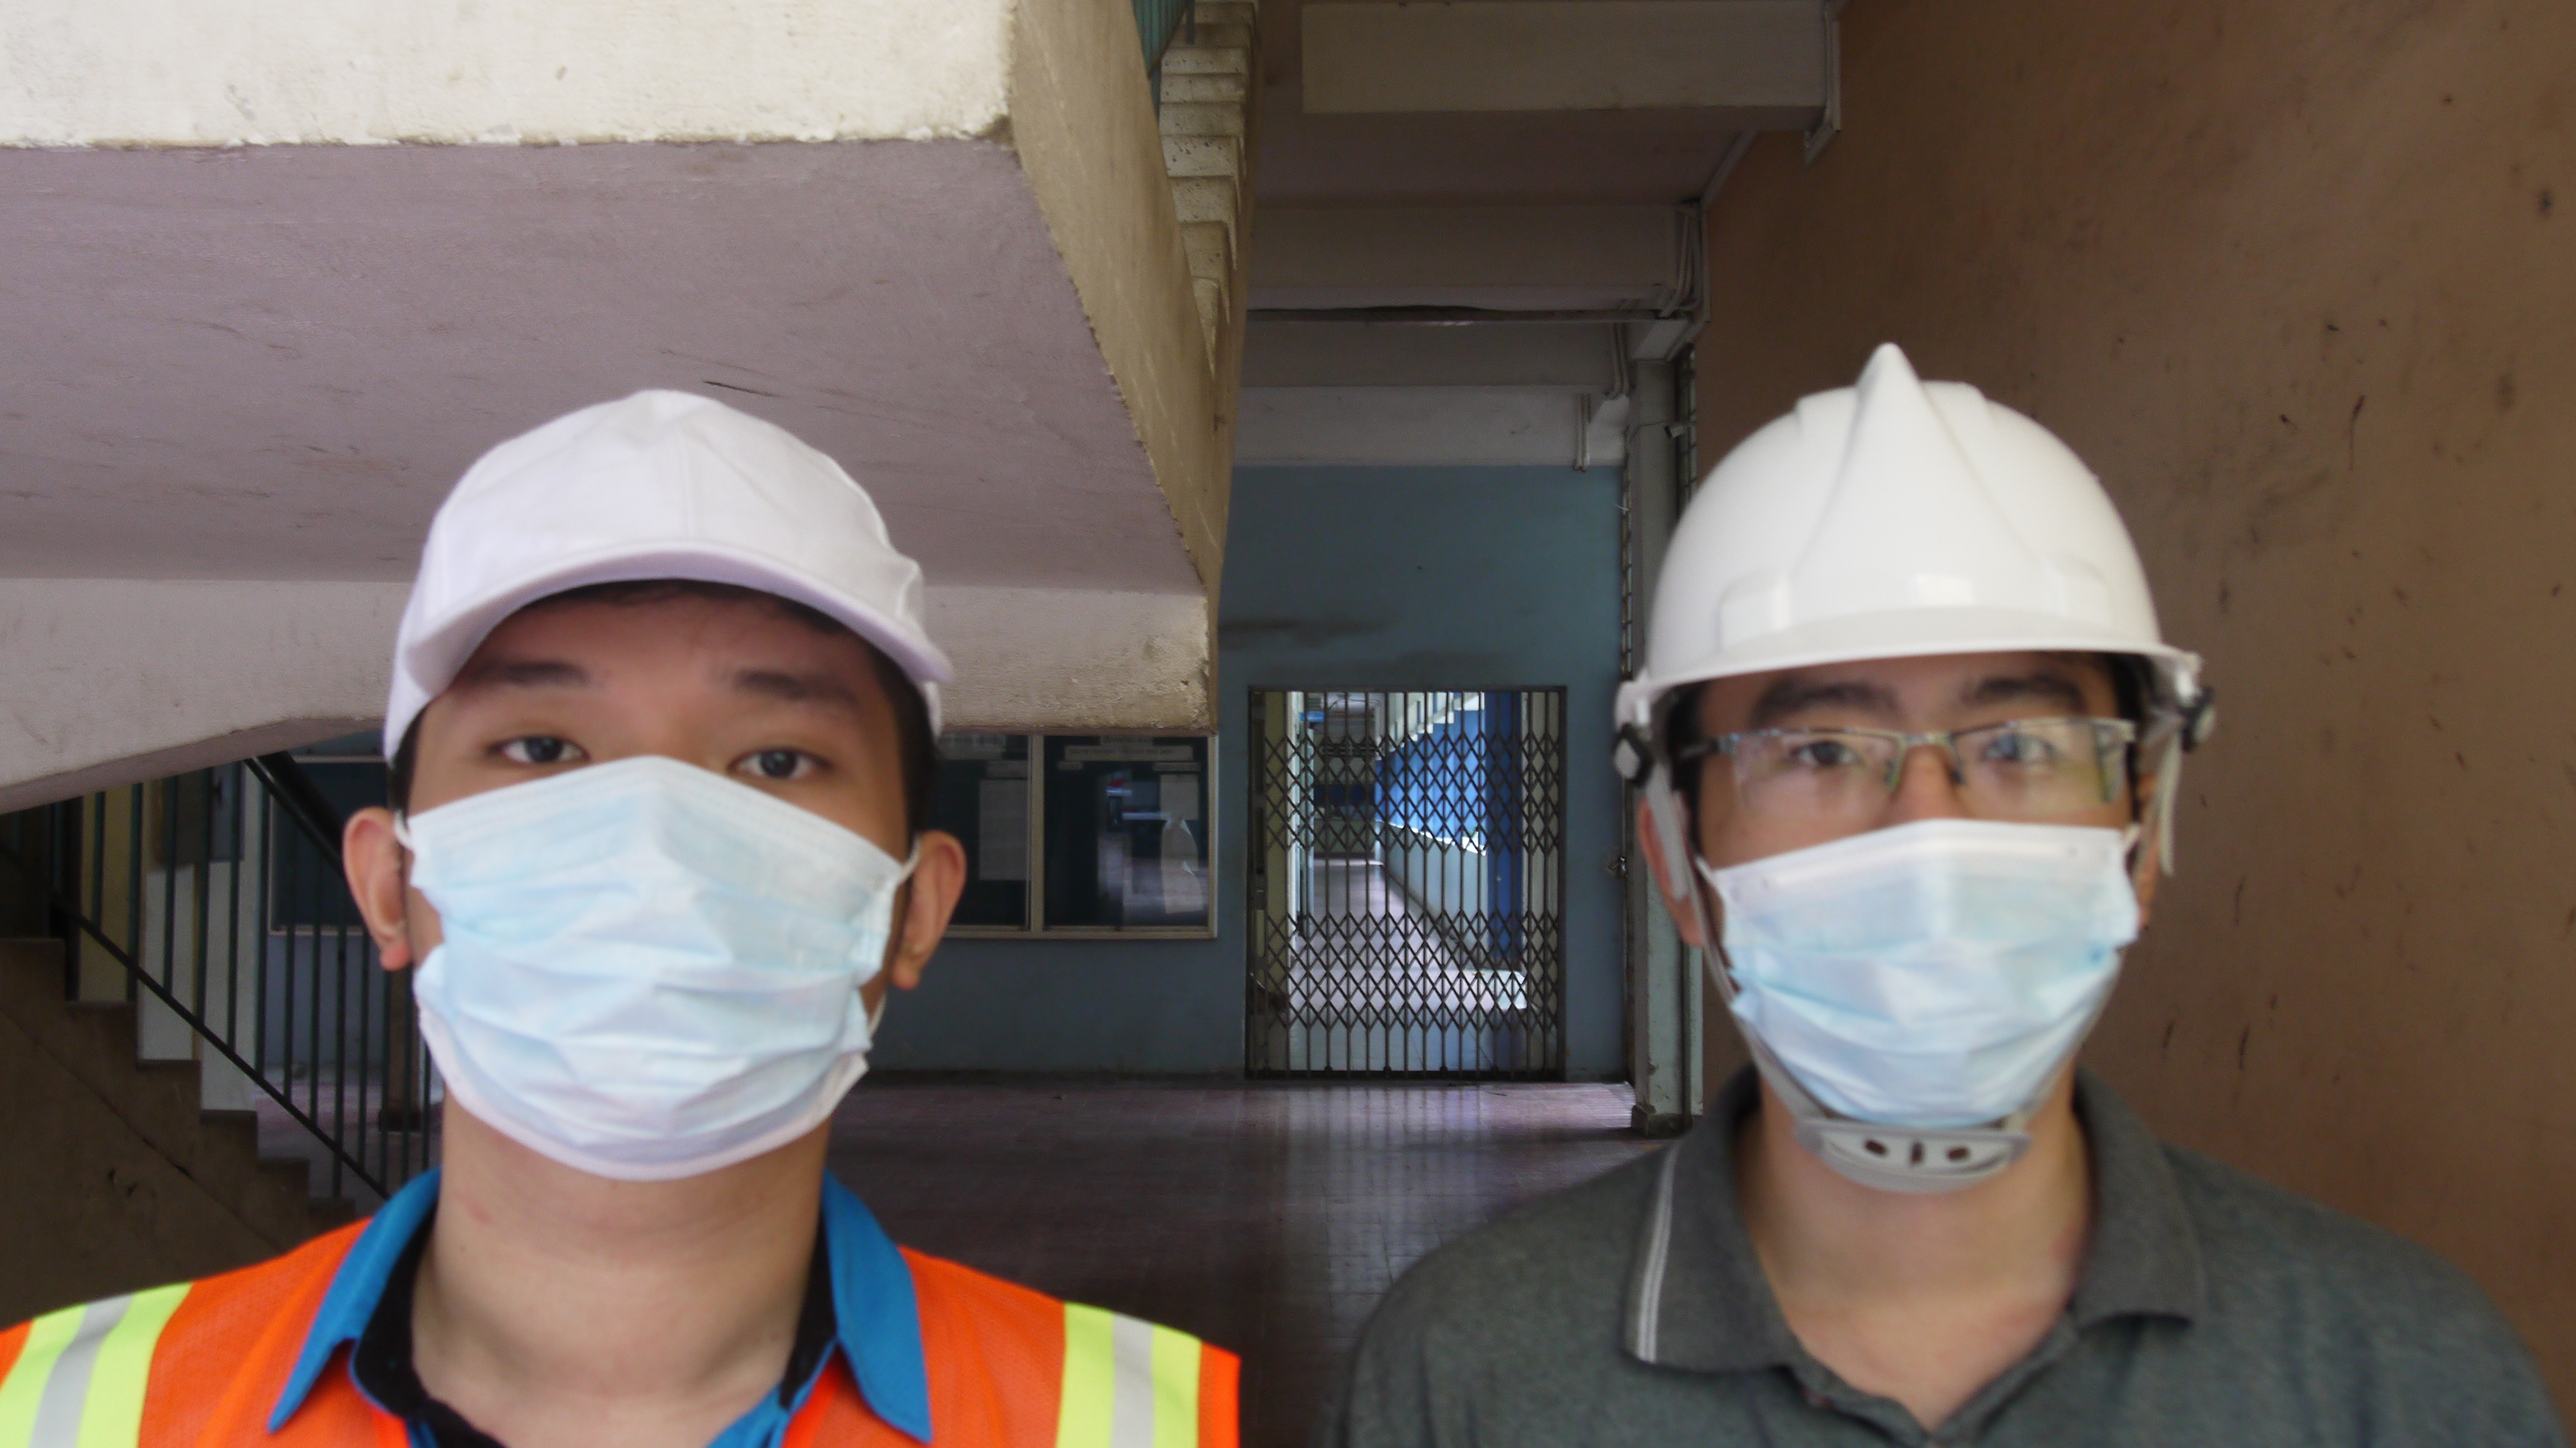
\includegraphics[width=\textwidth]{images/close1.JPG}
\caption{Một chủ thể đội nón vải trắng - bên trái và một chủ thể đội nón bảo hiểm trắng - bên phải. Góc chụp trực diện}
\label{fig:similar_white_hat_1}
\end{minipage}\hfill
\begin{minipage}{0.45\textwidth}
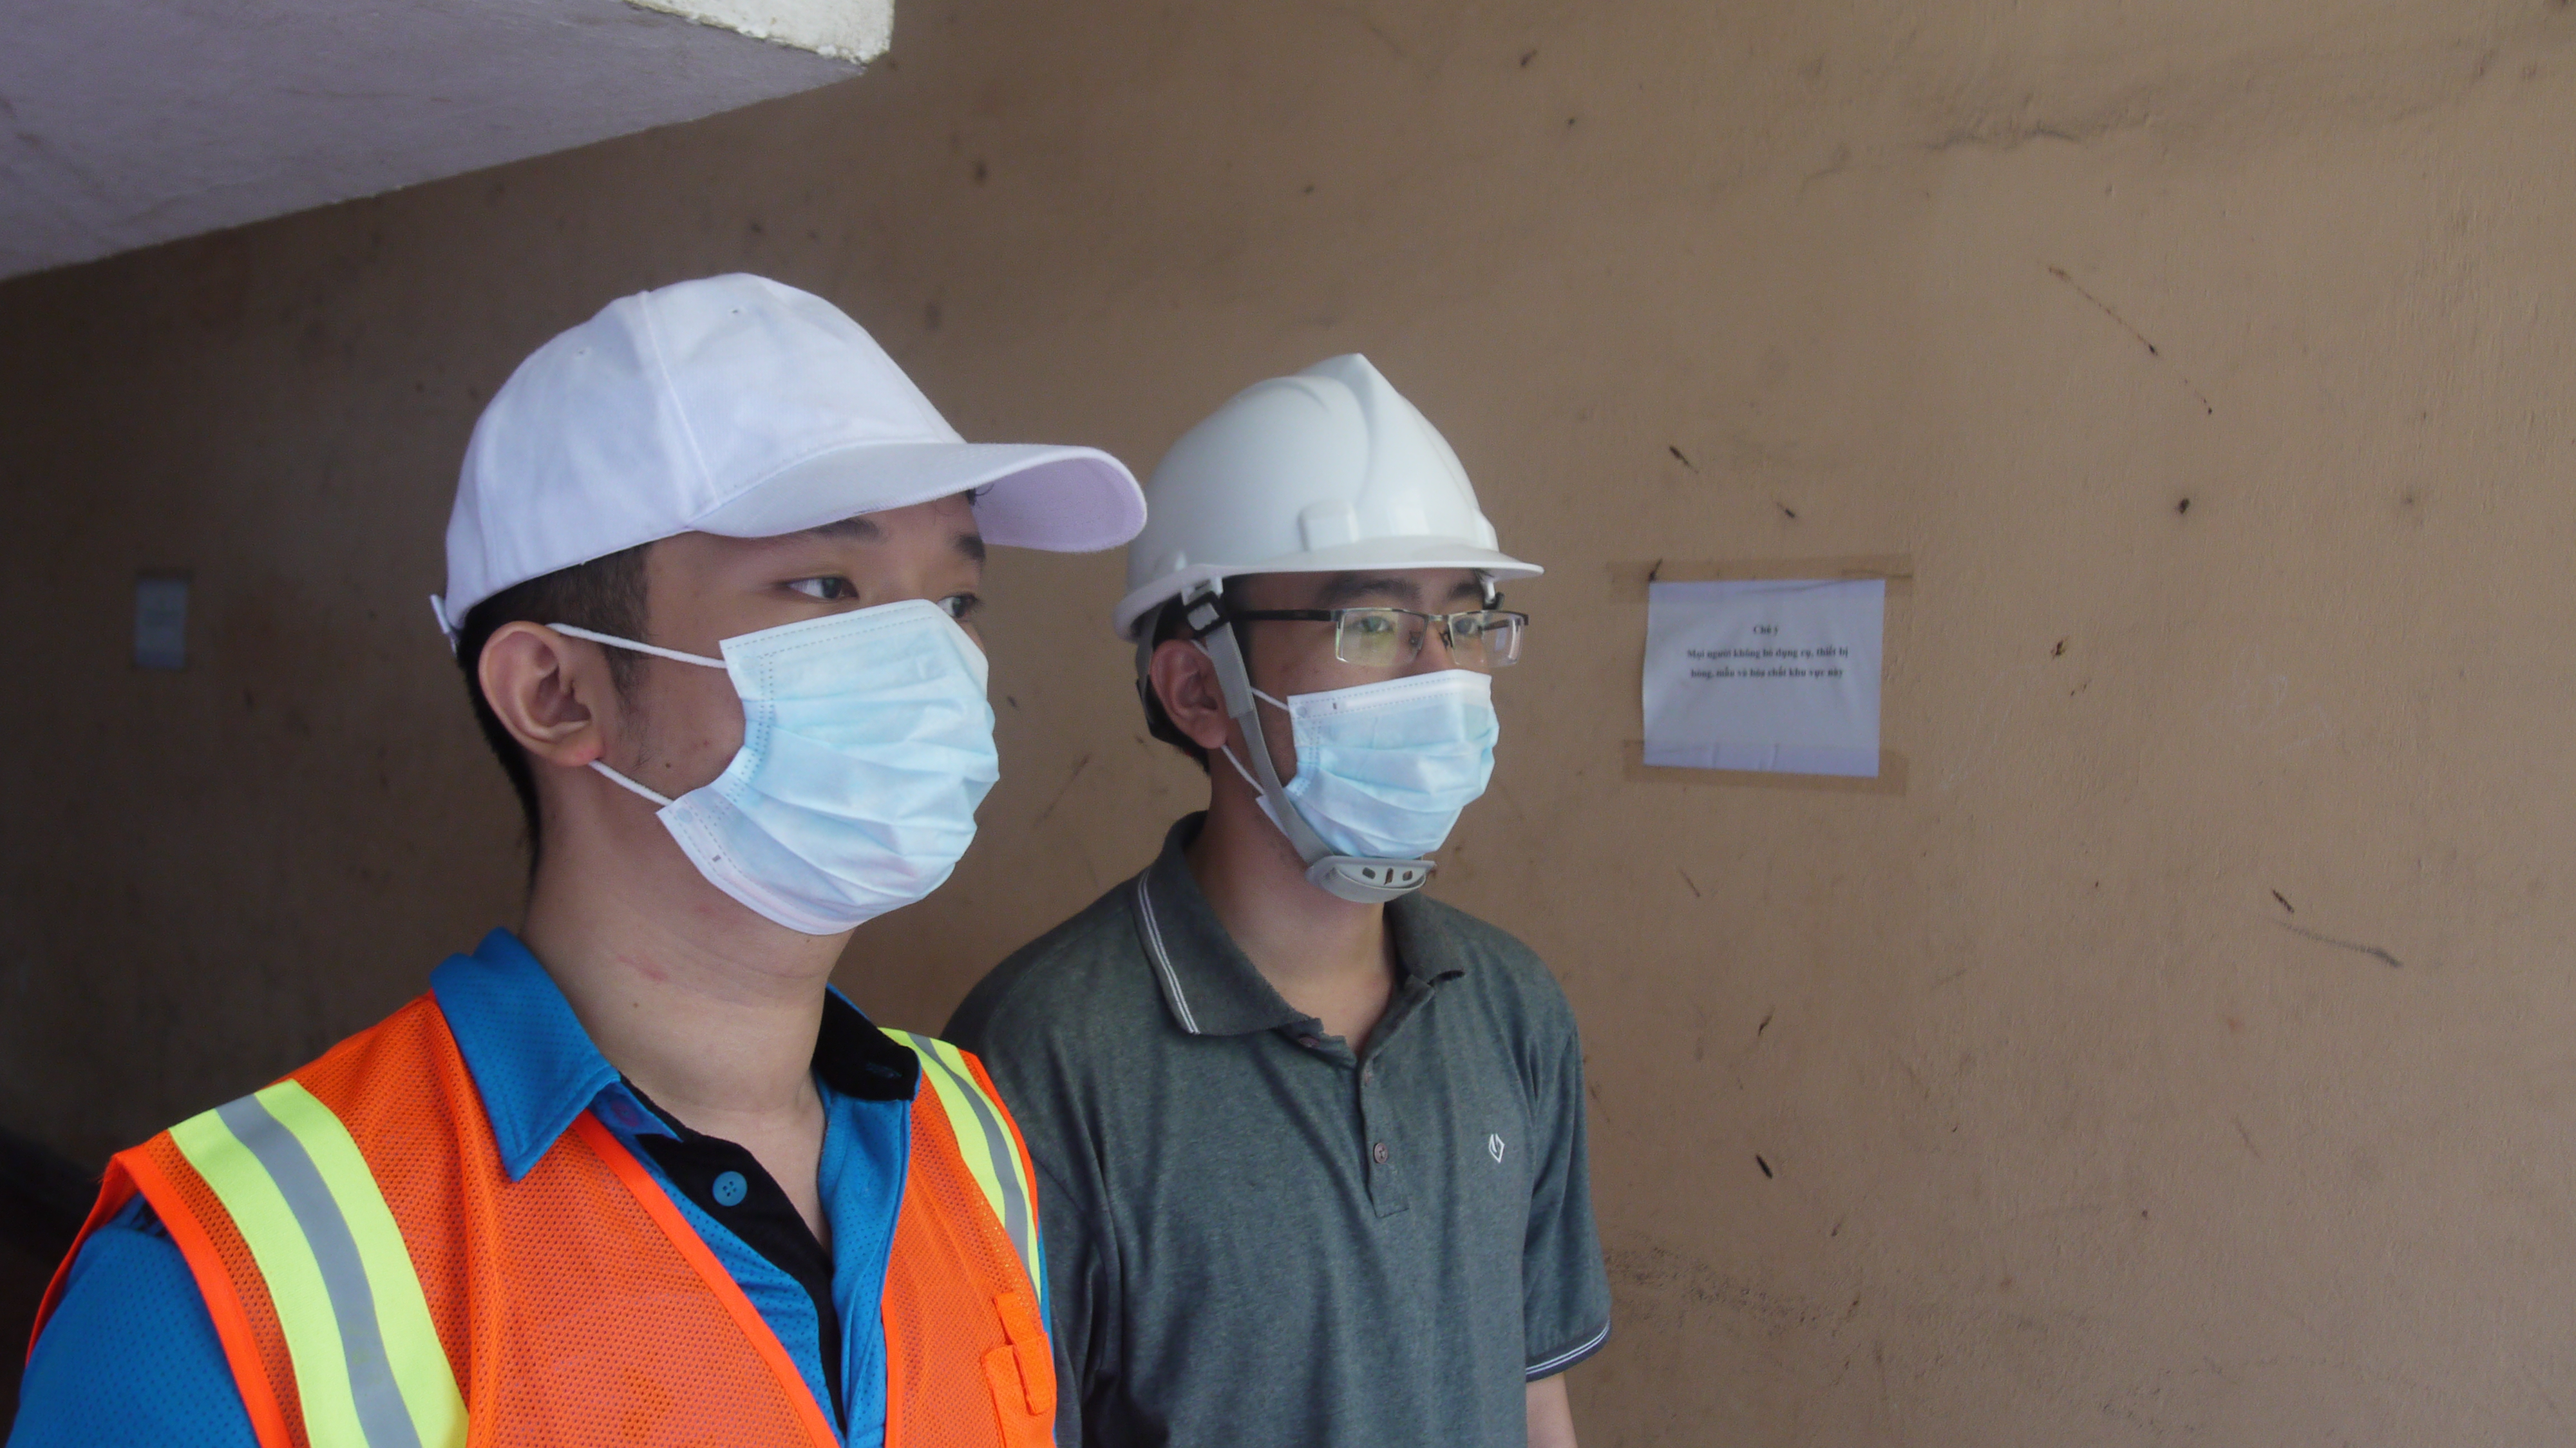
\includegraphics[width=\textwidth]{images/close2.JPG}
\caption{Một chủ thể đội nón vải trắng - bên trái và một chủ thể đội nón bảo hiểm trắng - bên phải. Góc chụp từ trái qua}
\label{fig:similar_white_hat_2}
\end{minipage}
\end{figure}

\emph{Kết quả}: Đồ thị precision ở hình \ref{fig:3_6_9_precision} và recall ở hình \ref{fig:3_6_9_recall} cho thấy mô hình hoạt động tốt nhất ở khoảng cách $6$m. Các thông số precision và recall của hầu hết các class ở $6$m đều trội hơn so với ở $3$m và $9$m. Việc precision cao sẽ giúp các dự đoán của mô hình tại $6$m chính xác hơn so với tại $3$m và $9$m. Recall cao nói lên rằng mô hình sẽ nhạy hơn và có thể phát hiện được nhiều vật thể hơn trong một khung hình tại khoảng cách $6$m. Tại class \emph{Not wearing a hardhat} có sự dao động về thông số hiệu năng và kết quả dự đoán ở khoảng cách $6$m vẫn chưa là tốt nhất điều này có thể xuất phát từ việc các bounding box của class \emph{Not wearing a hardhat} trong tập dữ liệu huấn luyện có kích thước gần tương đồng với các bounding box của vật thể cùng class ở khoảng cách $9$m.
\begin{figure}[ht!]
	\centerline{\includegraphics[scale=0.5]{images/3_6_9_precision.png}}
  	\caption{Precision của các class tại các khoảng cách {\color{red} 3m}, {\color{blue} $6$m}, {\color{black} $9$m}. Cao hơn nghĩa là tốt hơn.}
  	\label{fig:3_6_9_precision}
\end{figure}
\begin{figure}[ht!]
	\centerline{\includegraphics[scale=0.5]{images/3_6_9_recall.png}}
  	\caption{Recall của các class tại các khoảng cách {\color{red} 3m}, {\color{blue} $6$m}, {\color{black} $9$m}. Cao hơn nghĩa là tốt hơn.}
  	\label{fig:3_6_9_recall}
\end{figure}

Ngoài ra, mô hình cũng có thể phân biệt tốt giữa nón vải trắng và nón bảo hộ trắng tại khoảng cách $3$m như trên hình \ref{fig:good_hh} và \ref{fig:good_hh_zoom}. Tại $6$m mô hình vẫn tiếp tục phân biệt tốt như trên hình \ref{fig:good_hh_6m} và \ref{fig:good_hh_6m_zoom}. Độ chính xác giảm xuống khi chủ thể cách xa camera $9$m như trên hình \ref{fig:good_hh_9m} và \ref{fig:good_hh_9m_zoom}.
\begin{figure}[ht!]
	\centerline{\includegraphics[scale=0.1]{images/good_hh.jpg}}
  	\caption{Dự đoán của mô hình ở khoảng cách 3m.}
  	\label{fig:good_hh}
\end{figure}
\begin{figure}[ht!]
	\centerline{\includegraphics[scale=0.4]{images/good_hh_zoom.jpg}}
  	\caption{Mô hình có thể phân biệt tốt giữa nón vải trắng và nón bảo hiểm trắng ở khoảng cách 3m.}
  	\label{fig:good_hh_zoom}
\end{figure}
\begin{figure}[ht!]
	\centerline{\includegraphics[scale=0.1]{images/good_hh_6m.jpg}}
  	\caption{Dự đoán của mô hình ở khoảng cách 6m.}
  	\label{fig:good_hh_6m}
\end{figure}
\begin{figure}[ht!]
	\centerline{\includegraphics[scale=0.4]{images/good_hh_6m_zoom.jpg}}
  	\caption{Mô hình có thể phân biệt tốt giữa nón vải trắng và nón bảo hiểm trắng ở khoảng cách 6m.}
  	\label{fig:good_hh_6m_zoom}
\end{figure}
\begin{figure}[ht!]
	\centerline{\includegraphics[scale=0.1]{images/bad_hh_9m.jpg}}
  	\caption{Dự đoán của mô hình ở khoảng cách 9m.}
  	\label{fig:good_hh_9m}
\end{figure}
\begin{figure}[ht!]
	\centerline{\includegraphics[scale=0.8]{images/bad_hh_9m_zoom.jpg}}
  	\caption{Mô hình không thể phân biệt tốt giữa nón vải trắng và nón bảo hiểm trắng ở khoảng cách 9m.}
  	\label{fig:good_hh_9m_zoom}
\end{figure}

\subsubsection{Thử nghiệm khả năng nhận diện của mô hình vơi các trường hợp sử dụng sai cách các thiết bị bảo hộ}
Việc sử dụng các thiết bị bảo hộ sai cách cũng nguy hiểm giống như việc không sử dụng thiết bị bảo hộ, do đó không chỉ cần phải phân biệt giữa có sử dụng hay không mà mô hình còn phải có thể phân biệt được giữa sử dụng đúng và sai trang thiết bị bảo hộ. Trong trường hợp này, chủ thể sẽ đeo khẩu trang sai cách hoặc mặc áo phản quang sai cách để kiểm tra khả năng nhận diện của mô hình.

\emph{Trường hợp 1}: Việc đeo khẩu trang sai cách sẽ được thực hiện thông qua hai trường hợp, một là đeo khẩu trang hở mũi - hình \ref{fig:bad_mask_nose}, hai là đeo khẩu trang hở miệng - hình \ref{fig:bad_mask_mouth}. Các kết quả dự đoán được thực hiện trên hình ở khoảng cách $3$m.
\begin{figure}[ht!]
	\centerline{\includegraphics[scale=0.7]{images/bad_mask_nose.jpg}}
  	\caption{Chủ thể (bên trái) đeo khẩu trang không che kín mũi ở khoảng cách 3m.}
  	\label{fig:bad_mask_nose}
\end{figure}
\begin{figure}[ht!]
	\centerline{\includegraphics[scale=0.65]{images/bad_mask_mouth.jpg}}
  	\caption{Chủ thể (bên trái) đeo khẩu trang không che kín miệng ở khoảng cách 3m.}
  	\label{fig:bad_mask_mouth}
\end{figure}
\emph{Kết quả}: Mô hình không thể phân biệt được trường hợp đeo khẩu trang sai khi chủ thể đeo khẩu trang để hở mũi - hình \ref{fig:bad_mask_nose_pred}. Mô hình có thể phân biệt tốt trong trương hợp đeo khẩu trang sai khi chủ thể đeo khẩu trang hở miệng - hình \ref{fig:bad_mask_mouth_pred}.
\begin{figure}[ht!]
	\centerline{\includegraphics[scale=0.3]{images/bad_mask_nose_pred.jpg}}
  	\caption{Kết quả dự đoán không tốt với chủ thể (bên trái) đeo khẩu trang không che kín mũi ở khoảng cách 3m.}
  	\label{fig:bad_mask_nose_pred}
\end{figure}
\begin{figure}[ht!]
	\centerline{\includegraphics[scale=0.3]{images/bad_mask_mouth_pred.jpg}}
  	\caption{Kết quả dự đoán tốt với chủ thể (bên trái) đeo khẩu trang không che kín miệng ở khoảng cách 3m.}
  	\label{fig:bad_mask_mouth_pred}
\end{figure}

\emph{Trường hợp 2}: Việc mặc áo bảo hộ sai cách sẽ được thực hiện bằng cách chỉ đặt áo lên người mà không thật sự mặc hoặc mặc nhưng không cài vào đúng cách như trong hình \ref{fig:bad_sv}, việc này có thể khiến áo dễ mắc vào các thiết bị phương tiện đang hoạt động và gây ra các tai nạn đáng tiếc. Các kết quả dự đoán được thực hiện trên hình ở khoảng cách $3$m.
\begin{figure}[ht!]
	\centerline{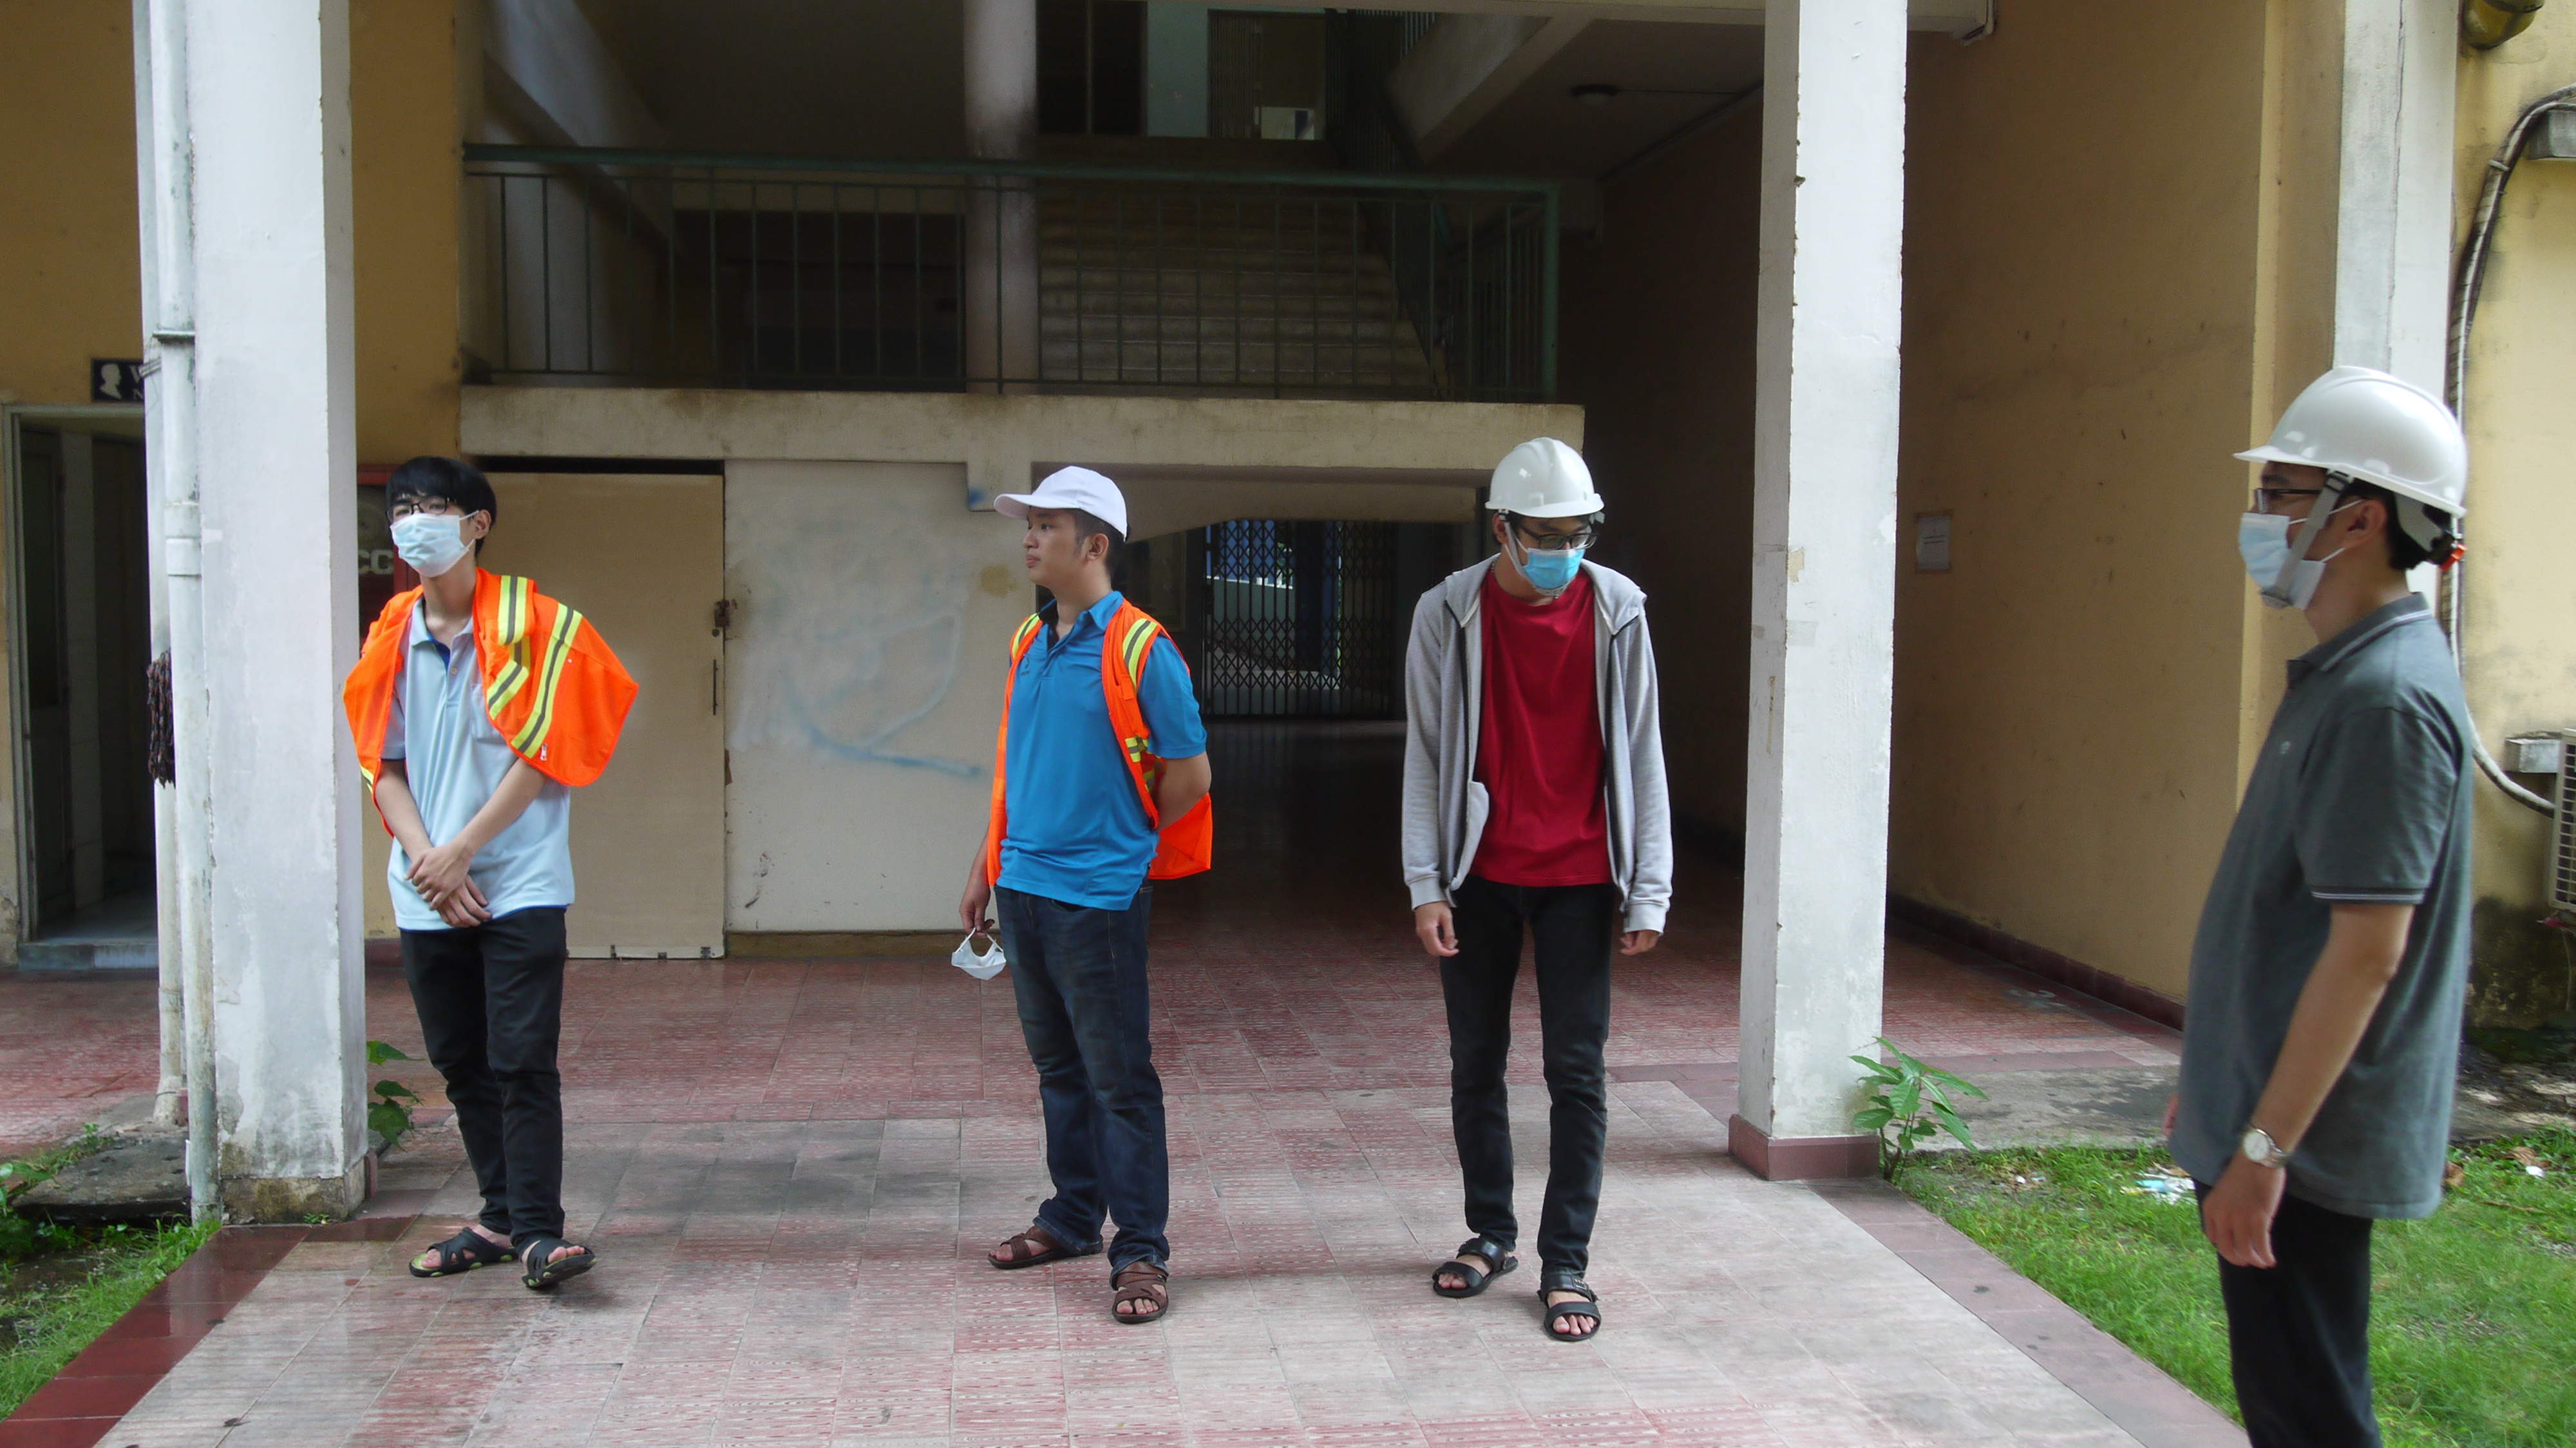
\includegraphics[scale=0.25]{images/bad_sv.jpg}}
  	\caption{Hai chủ thể (bên trái ngoài cùng) mặc áo bảo hộ sai cách ở khoảng cách 3m.}
  	\label{fig:bad_sv}
\end{figure}
\emph{Kết quả}: Mô hình có thể phân biệt được các trường hợp mặc sai áo bảo hộ ở phần lớn các trường hợp như trên hình \ref{fig:bad_sv_pred_1} và \ref{fig:bad_sv_pred_2}. Tuy nhiên ở một vài góc chụp như trên hình \ref{fig:bad_sv_pred_3} thì mô hình không thể nhận diện được chính xác. Điều này có thể không phải là nhược điểm lớn vì khi nhận diện trong thực tế thì mô hình sẽ nhận diện liên tục qua nhiều khung hình do đó những trường hợp mặc sai khi bị bỏ qua ở khung hình này thì sẽ được phát hiện trong khung hình khác.
\begin{figure}[ht!]
	\centerline{\includegraphics[scale=0.18]{images/bad_sv_predict_2.jpg}}
  	\caption{Kết quả dự đoán tốt với hai chủ thể mặc áo bảo hộ sai cách ở khoảng cách 3m.}
  	\label{fig:bad_sv_pred_1}
\end{figure}
\begin{figure}[ht!]
	\centerline{\includegraphics[scale=0.35]{images/bad_sv_predict_3.jpg}}
  	\caption{Kết quả dự đoán tốt với hai chủ thể mặc áo bảo hộ sai cách (góc máy khác) ở khoảng cách 3m.}
  	\label{fig:bad_sv_pred_2}
\end{figure}
\begin{figure}[ht!]
	\centerline{\includegraphics[scale=0.18]{images/bad_sv_predict_4.jpg}}
  	\caption{Kết quả dự đoán không tốt với hai chủ thể mặc áo bảo hộ sai cách ở khoảng cách 3m.}
  	\label{fig:bad_sv_pred_3}
\end{figure}\newpage\cleardoublepage
\chapter{Kết luận}
In this chapter, ...\newpage\cleardoublepage

\nocite{*}
\bibliography{references}\newpage\cleardoublepage
\bibliographystyle{plain}
\end{document}